\documentclass[a4paper,oneside]{../../styles/thesis}
\usepackage[utf8]{vietnam}
\renewcommand{\rmdefault}{utm}
\renewcommand{\sfdefault}{uhv}
\renewcommand{\ttdefault}{ucr}
\usepackage[unicode,hidelinks]{hyperref}
%\setmathfont{Asana-Math}
\usepackage{fix-cm}
\usepackage{color}
%\usepackage{lyk-z13}
%\usepackage[unicode]{hyperref}
\usepackage{amscd,amssymb}
%\usepackage{array} % Load array package before xy-pic to avoid conflicts
%\usepackage[v2,cmtip]{xy} % Commented out due to conflicts with array package
\usepackage{urwchancal}
\usepackage{amsthm}
\usepackage{rotating}
%%%%%%%%%%%%%%%%%

\usepackage{longfbox}%gGói lệnh đóng khung văn bản đẹp
\usepackage{listings}
\usepackage{mathptmx}
\usepackage{subfig}
\usepackage{colortbl}
\usepackage{graphicx}
\usepackage{array} % Needed for p{...} column types in tabular
\usepackage{multicol}
\usepackage{longtable}
\usepackage{indentfirst}
\usepackage{makeidx}
\usepackage{xspace}
\usepackage{titlesec}
\usepackage{multicol}
%\usepackage{pb-diagram}
\usepackage{titletoc}
\usepackage{fancyhdr}

% Định dạng tiêu đề chương
\titleformat{\chapter}[display]
{\normalfont\huge\bfseries\centering}
{\chaptertitlename\ \thechapter}{20pt}{\Huge}

% Định dạng tiêu đề section
\titleformat{\section}
{\normalfont\Large\bfseries}
{\thesection}{1em}{}

% Định dạng tiêu đề subsection
\titleformat{\subsection}
{\normalfont\large\bfseries}
{\thesubsection}{1em}{}
%\usepackage{glossaries}
 %\usepackage{maybemath}
%\usepackage{aliascnt}
\usepackage{wallpaper} 
\usepackage{fancybox}
\usepackage {imakeidx}
\input ../../styles/vietnamese-typeset.tex
%\input diagxy
\newlength{\defbaselineskip}
\setlength{\defbaselineskip}{\baselineskip}
\newcommand{\setlinespacing}[1]%
           {\setlength{\baselineskip}{#1 \defbaselineskip}}
\newcommand{\doublespacing}{\setlength{\baselineskip}%
                           {2.0 \defbaselineskip}}
\newcommand{\singlespacing}{\setlength{\baselineskip}{\defbaselineskip}}
\renewcommand{\sectionmark}[1]{\markright{\small{\textit{\thesection. #1}}}{}}

% Cấu hình header và footer
\pagestyle{fancy}
\fancyhf{} % Xóa tất cả header và footer
\fancyhead[L]{\small\leftmark} % Header trái: tên chương
\fancyhead[R]{\small\rightmark} % Header phải: tên section
\fancyfoot[C]{\thepage} % Footer giữa: số trang
\renewcommand{\headrulewidth}{0.4pt} % Đường kẻ dưới header
\renewcommand{\footrulewidth}{0pt} % Không có đường kẻ trên footer

% Định dạng cho trang đầu chương
\fancypagestyle{plain}{
    \fancyhf{}
    \fancyfoot[C]{\thepage}
    \renewcommand{\headrulewidth}{0pt}
    \renewcommand{\footrulewidth}{0pt}
}

% Chen code Matlab
\usepackage{listings}
\definecolor{dkgreen}{rgb}{0,0.6,0}
\definecolor{gray}{rgb}{0.5,0.5,0.5}
\definecolor{mauve}{rgb}{0.58,0,0.82}

\lstset{frame=tb,
 language=matlab,
 aboveskip=3mm,
 belowskip=3mm,
 showstringspaces=false,
 columns=flexible,
 basicstyle={\small\ttfamily},
 numbers=none,
 numberstyle=\tiny\color{gray},
 keywordstyle=\color{blue},
 commentstyle=\color{dkgreen},
 stringstyle=\color{mauve},
 breaklines=true,
 breakatwhitespace=true,
 tabsize=3
}
\newtheorem{matlab}{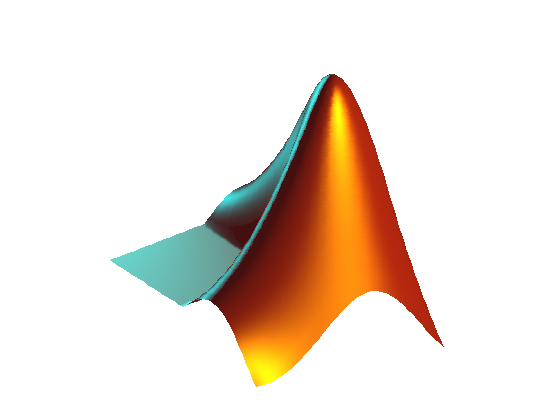
\includegraphics[scale=.11,bb= 500 300 50 250]{../../assets/logos/matlab-logo.png}M.}[chapter]




%%%%%%%%%%%%%



\begin{document}


%%%%%%%%%%%%%%%% BIA 
%\renewcommand{\normalsize}{\fontsize{13}{18}\selectfont}
\fontsize{13pt}{22pt}\selectfont
%\dominitoc
%\pagestyle{myheadings}
%\pagenumbering{arabic}
\ThisCenterWallPaper{1}{../../assets/images/background-frame-4.png}

\thispagestyle{empty}
\begin{titlepage}

\hspace{2.8cm} {\bf \fontsize{16pt}{16}\selectfont TRƯỜNG ĐẠI HỌC CẦN THƠ}\\
\vspace*{0.05cm}
\hspace{3.3cm} {\bf\fontsize{16pt}{16}\selectfont KHOA KHOA HỌC TỰ NHIÊN}\\
 \vspace*{0.05cm}
\hspace{4.3cm} {\bf\fontsize{16pt}{16}\selectfont BỘ MÔN TOÁN HỌC}\\

\begin{figure}[h!]
\hspace{5cm} 
\includegraphics[width=40mm]{../../assets/logos/university-logo.png}
\end{figure}

\vspace*{0.5cm}

\hspace{4cm}{\bf\fontsize{16pt}{20}\selectfont BÀI THU HOẠCH}\\
 \vspace*{0.05cm}\\
\vspace*{2cm}

\begin{center}
 {\bf\fontsize{20pt}{28}\selectfont CHUYÊN ĐỀ THỐNG KÊ NÂNG CAO}   
\end{center}




\vspace*{1.5cm}

\begin{center}
\textbf{Sinh viên thực hiện}\\    
\textbf{TRẦN VĂN LÝ }\\
\textbf{NGÀNH LTXS \& TKTH - Khóa 31}\\
\textbf{MSHV: 001111}
\end{center}



\vspace*{3cm}
\hspace{4.0cm}{\bf \fontsize{16pt}{18}\selectfont CẦN THƠ - NĂM 2025}
\end{titlepage}



\newpage

%%% LOT BIA

\begin{titlepage}

\hspace{2.8cm} {\bf \fontsize{16pt}{16}\selectfont TRƯỜNG ĐẠI HỌC CẦN THƠ}\\
\vspace*{0.05cm}
\hspace{3.3cm} {\bf\fontsize{16pt}{16}\selectfont KHOA KHOA HỌC TỰ NHIÊN}\\
 \vspace*{0.05cm}
\hspace{4.3cm} {\bf\fontsize{16pt}{16}\selectfont BỘ MÔN TOÁN HỌC}\\
\vspace*{0.05cm}
\hspace{5 cm} <><><><><><><><> 


\vspace*{2cm}

\hspace{4cm}{\bf\fontsize{16pt}{20}\selectfont BÀI THU HOẠCH}\\
 \vspace*{0.05cm}\\
\vspace*{2cm}

\begin{center}
 {\bf\fontsize{20pt}{28}\selectfont CHUYÊN ĐỀ THỐNG KÊ NÂNG CAO }   
\end{center}




\vspace*{1.5cm}

\begin{center}
\textbf{Sinh viên thực hiện}\\    
\textbf{TRẦN VĂN LÝ}\\
\textbf{NGÀNH LTXS \& TKTH - Khóa 31}\\
\textbf{MSHV: 001111}
\end{center}



\vspace*{3cm}
\hspace{4.0cm}{\bf \fontsize{16pt}{18}\selectfont CẦN THƠ - NĂM 2025}
\end{titlepage}

%%%%%%%%%%%%%%%%%%%%%%%%%%%%%%%%%%%%
% Bắt đầu phần mở đầu với số trang La Mã
\pagenumbering{roman}
\setlinespacing{1.3}

% Áp dụng style cho các trang mở đầu
\pagestyle{plain}

% Lời cảm ơn
\chapter*{LỜI CẢM ƠN}
\addcontentsline{toc}{chapter}{LỜI CẢM ƠN}

Em xin chân thành cảm ơn TS. Trần Văn Lý đã tận tình hướng dẫn và giúp đỡ em trong quá trình thực hiện bài thu hoạch này. Thầy đã truyền đạt những kiến thức quý báu về thống kê nâng cao và các phương pháp phân tích dữ liệu, giúp em hiểu sâu sắc hơn về các kỹ thuật kiểm định thống kê và phân tích đa biến.

Em cũng xin gửi lời cảm ơn đến các thầy cô trong Bộ môn Toán học, Khoa Khoa học Tự nhiên, Trường Đại học Cần Thơ đã tạo điều kiện thuận lợi cho việc học tập và nghiên cứu.

Cuối cùng, em xin cảm ơn gia đình và bạn bè đã động viên và hỗ trợ em trong suốt quá trình học tập.

\vspace{2cm}
\hfill\begin{minipage}{6cm}
\centering
Cần Thơ, tháng 12 năm 2024\\
Sinh viên\\[2ex]
\textbf{TRẦN TRUNG TÍN}
\end{minipage}

\newpage

% Mục lục
\tableofcontents
\newpage

% Danh sách hình vẽ
\addcontentsline{toc}{chapter}{\textbf{DANH SÁCH HÌNH VẼ}}
\listoffigures
\newpage

% Danh sách bảng
\addcontentsline{toc}{chapter}{\textbf{DANH SÁCH BẢNG}}
\listoftables
\newpage

% Danh sách ký hiệu và viết tắt
\chapter*{DANH SÁCH KÝ HIỆU VÀ VIẾT TẮT}
\addcontentsline{toc}{chapter}{DANH SÁCH KÝ HIỆU VÀ VIẾT TẮT}

\section*{Ký hiệu toán học cơ bản}
\begin{longtable}{@{}p{3cm}p{10cm}@{}}
\textbf{Ký hiệu} & \textbf{Ý nghĩa} \\
\hline
\endhead
$\Omega$ & Không gian mẫu \\
$\mathcal{F}$ & $\sigma$-đại số các biến cố \\
$P$ & Độ đo xác suất \\
$X, Y, Z$ & Biến ngẫu nhiên \\
$\mathbf{X}$ & Vector ngẫu nhiên \\
$x, y, z$ & Giá trị quan sát của biến ngẫu nhiên \\
$f_X(x)$ & Hàm mật độ xác suất (PDF) \\
$F_X(x)$ & Hàm phân phối tích lũy (CDF) \\
$F_n(x)$ & Hàm phân phối thực nghiệm (ECDF) \\
$\mathbb{E}[X]$ & Kỳ vọng của biến ngẫu nhiên $X$ \\
$\text{Var}(X)$ & Phương sai của biến ngẫu nhiên $X$ \\
$\text{Cov}(X,Y)$ & Hiệp phương sai giữa $X$ và $Y$ \\
$\rho_{XY}$ & Hệ số tương quan giữa $X$ và $Y$ \\
$\sigma$ & Độ lệch chuẩn tổng thể \\
$\sigma^2$ & Phương sai tổng thể \\
$\mu$ & Trung bình tổng thể \\
$\boldsymbol{\mu}$ & Vector kỳ vọng \\
$\boldsymbol{\Sigma}$ & Ma trận hiệp phương sai \\
$\mathbf{R}$ & Ma trận tương quan \\
$n$ & Kích thước mẫu \\
$\overline{X}$ & Trung bình mẫu \\
$S^2$ & Phương sai mẫu \\
$S$ & Độ lệch chuẩn mẫu \\
\end{longtable}

\section*{Ký hiệu phân phối xác suất}
\begin{longtable}{@{}p{3cm}p{10cm}@{}}
\textbf{Ký hiệu} & \textbf{Ý nghĩa} \\
\hline
\endhead
$\mathcal{N}(\mu,\sigma^2)$ & Phân phối chuẩn với trung bình $\mu$ và phương sai $\sigma^2$ \\
$\mathcal{N}_p(\boldsymbol{\mu},\boldsymbol{\Sigma})$ & Phân phối chuẩn nhiều chiều \\
$\chi^2(n)$ & Phân phối Chi-bình phương với $n$ bậc tự do \\
$t(n)$ & Phân phối Student với $n$ bậc tự do \\
$F(n_1,n_2)$ & Phân phối F với bậc tự do $(n_1,n_2)$ \\
$\text{B}(n,p)$ & Phân phối nhị thức với tham số $n$ và $p$ \\
$\text{Poisson}(\lambda)$ & Phân phối Poisson với tham số $\lambda$ \\
$U(a,b)$ & Phân phối đều trên đoạn $[a,b]$ \\
$\text{Exp}(\lambda)$ & Phân phối mũ với tham số $\lambda$ \\
$\text{Gamma}(\alpha,\beta)$ & Phân phối Gamma với tham số hình dạng $\alpha$ và tỷ lệ $\beta$ \\
\end{longtable}

\section*{Ký hiệu kiểm định thống kê}
\begin{longtable}{@{}p{3cm}p{10cm}@{}}
\textbf{Ký hiệu} & \textbf{Ý nghĩa} \\
\hline
\endhead
$H_0$ & Giả thuyết không (null hypothesis) \\
$H_1$ & Giả thuyết đối (alternative hypothesis) \\
$\alpha$ & Mức ý nghĩa (significance level) \\
$\beta$ & Xác suất sai lầm loại II \\
$1-\beta$ & Lực kiểm định (power of test) \\
$p$-value & Giá trị $p$ (probability value) \\
$\chi^2_{\text{obs}}$ & Giá trị quan sát của thống kê Chi-bình phương \\
$D_n$ & Thống kê Kolmogorov-Smirnov \\
$O_i$ & Tần số quan sát (observed frequency) \\
$E_i$ & Tần số kỳ vọng (expected frequency) \\
$z_{\alpha}$ & Phân vị chuẩn tại mức $\alpha$ \\
$t_{\alpha,n}$ & Phân vị Student tại mức $\alpha$ với $n$ bậc tự do \\
$\chi^2_{\alpha,n}$ & Phân vị Chi-bình phương tại mức $\alpha$ với $n$ bậc tự do \\
\end{longtable}

\section*{Ký hiệu phân tích nhiều chiều}
\begin{longtable}{@{}p{3cm}p{10cm}@{}}
\textbf{Ký hiệu} & \textbf{Ý nghĩa} \\
\hline
\endhead
$\mathbf{A}$ & Ma trận các vector riêng trong PCA \\
$\boldsymbol{\Lambda}$ & Ma trận chéo các trị riêng \\
$\lambda_i$ & Trị riêng thứ $i$ \\
$\mathbf{a}_i$ & Vector riêng thứ $i$ \\
$Y_i$ & Thành phần chính thứ $i$ \\
$\mathbf{L}$ & Ma trận tải nhân tố (factor loading matrix) \\
$\mathbf{F}$ & Vector nhân tố chung \\
$\boldsymbol{\epsilon}$ & Vector sai số cụ thể \\
$\boldsymbol{\Psi}$ & Ma trận phương sai cụ thể \\
$h_i^2$ & Phương sai chung (communality) của biến thứ $i$ \\
$\psi_i$ & Phương sai cụ thể (specific variance) của biến thứ $i$ \\
$KMO$ & Chỉ số Kaiser-Meyer-Olkin \\
$MSA$ & Measure of Sampling Adequacy \\
\end{longtable}

\section*{Ký hiệu hội tụ và giới hạn}
\begin{longtable}{@{}p{3cm}p{10cm}@{}}
\textbf{Ký hiệu} & \textbf{Ý nghĩa} \\
\hline
\endhead
$\xrightarrow{P}$ & Hội tụ theo xác suất \\
$\xrightarrow{a.s.}$ & Hội tụ hầu chắc chắn \\
$\xrightarrow{\mathcal{D}}$ & Hội tụ theo phân phối \\
$\Rightarrow$ & Hội tụ yếu (weak convergence) \\
$\overset{d}{\approx}$ & Xấp xỉ theo phân phối \\
$\overset{i.i.d.}{\sim}$ & Độc lập cùng phân phối \\
$\mathbf{1}_A$ & Hàm chỉ báo của tập $A$ \\
$\sup$ & Supremum (cận trên nhỏ nhất) \\
$\inf$ & Infimum (cận dưới lớn nhất) \\
\end{longtable}

\section*{Viết tắt và thuật ngữ}
\begin{longtable}{@{}p{4cm}p{9cm}@{}}
\textbf{Viết tắt} & \textbf{Ý nghĩa} \\
\hline
\endhead
\textbf{Lý thuyết xác suất} & \\
LTXS & Lý thuyết xác suất \\
TKTH & Thống kê toán học \\
CLT & Central Limit Theorem (Định lý giới hạn trung tâm) \\
LLN & Law of Large Numbers (Luật số lớn) \\
CDF & Cumulative Distribution Function (Hàm phân phối tích lũy) \\
PDF & Probability Density Function (Hàm mật độ xác suất) \\
PMF & Probability Mass Function (Hàm khối xác suất) \\
ECDF & Empirical Cumulative Distribution Function \\
\\
\textbf{Kiểm định thống kê} & \\
GOF & Goodness of Fit (Kiểm định tính phù hợp) \\
K-S & Kolmogorov-Smirnov \\
MRF & Markov Random Field \\
\\
\textbf{Phân tích nhiều chiều} & \\
PCA & Principal Component Analysis (Phân tích thành phần chính) \\
FA & Factor Analysis (Phân tích nhân tố) \\
EFA & Exploratory Factor Analysis (Phân tích nhân tố khám phá) \\
CFA & Confirmatory Factor Analysis (Phân tích nhân tố khẳng định) \\
KMO & Kaiser-Meyer-Olkin \\
MSA & Measure of Sampling Adequacy \\
ML & Maximum Likelihood (Cực đại hóa likelihood) \\
\\
\textbf{Công cụ và phần mềm} & \\
MATLAB & Matrix Laboratory \\
SPSS & Statistical Package for the Social Sciences \\
SAS & Statistical Analysis System \\
\\
\textbf{Tổ chức} & \\
CTU & Can Tho University (Trường Đại học Cần Thơ) \\
ĐHCT & Đại học Cần Thơ \\
KHTN & Khoa Học Tự Nhiên \\
\end{longtable}

\newpage

%%%%%%%%%%%%%%%%%%%%%%%%%%%%%%%%%%%%
% Bắt đầu nội dung chính với số trang Ả-rập
\pagenumbering{arabic}
\setcounter{page}{1}
\setlinespacing{1.5}

% Áp dụng style fancy cho nội dung chính
\pagestyle{fancy}

% Phần mở đầu
\lmd
\textbf{1. Lý do chọn đề tài}



\textbf{2. Mục tiêu và phạm vi nghiên cứu}

\textbf{2.1. Mục tiêu nghiên cứu}

\textbf{2.2. Phạm vi nghiên cứu}

\textbf{3. Phương pháp nghiên cứu}



\textbf{4. Cấu trúc của luận văn}



\hspace{.5cm}


% Các chương chính
\chapter{Kiến thức chuẩn bị}
\setcounter{page}{1}
\pagenumbering{arabic}
Nội dung này được tham khảo và tổng hợp từ các tài liệu tham khảo \cite{1}, \cite{2} và \cite{5}. 


\section{Mục 1 không có dấu chấm cuối dòng}
\subsection{Tiểu mục 1 không có dấu chấm cuối dòng}

Mỗi đoạn diễn đạt cho mỗi ý bao gồm nhiều câu. Mỗi câu phải đầy đủ cú pháp: S + V + O (nếu có).

Qua đoạn mới phải thụt đầu dòng bằng cách chừa 1 dòng trống trong Latex. Thông thường người ta rất hạn chế sử dụng $\setminus\setminus$ để xuống dòng. 
\begin{dn}
 Nội dung định nghĩa viết vào đây
\end{dn}

\[ \int_{x=0}^5 f_X (x) {\rm d}x=1 \]

\begin{dn}
 Nội dung định nghĩa viết vào đây có thể sửa lại
\end{dn}

\begin{dl}
 Nội dung định lý viết vào đây   
\end{dl}

\cm{
Nội dung CM viết vào đây.
}

\subsection{Tiểu mục 2}
%%%%%%%%%Chèn bảng

\begin{table}[ht]
 \caption{\textbf{Bảng minh họa 1}}
    \centering
    \begin{tabular}{|c|c|c|c|c|}
    \hline
     STT    & Họ và tên & Kiểm tra & Thi & Tổng\\
      \hline
     1    & Nguyễn Văn A &  &  & \\
      \hline
      2   &  &  &  & \\
       \hline
         &  &  &  & \\
       \hline
    \end{tabular} 
    %\label{tab:my_label}
\end{table}

%%%%%%%%%%%%%Dạng tùy chỉnh kích thước cột
\begin{table}[ht]
 \caption{\textbf{Bảng minh họa 2}}
 \centering
\begin{tabular}{|c|l|l|l|c|c|}
		\hline
		\textbf{Stt} &\textbf{Tên bài báo} & \textbf{Tác giả/nhóm tác giả}
		& \textbf{Tên tạp chí} &\textbf{Số tạp chí} & \textbf{Năm xuất bản}
		\\
		\hline
		1 &   &  & &  & \\
		\hline
	2 &   &  & &  & \\
		\hline
        3 &   &  & &  & \\
		\hline
	\end{tabular}
    \end{table}
%%%%%%%%%%%%%%%%%%%%%%%%%%%%%%%%%%%%%%%%%%%%%%%%%%
% nội dung này có thể tham khảo giáo trình ĐSTT và HH2
\section{Mục 2}
\subsection{Tiểu mục 1}

\subsection{Tiểu mục 2}




\chapter{Một số dạng kiểm định thống kê}




\section{Kiểm đinh Pearson}
\subsection{Hàm phân phối tích luỹ}
\begin{dn}
 Nội dung định nghĩa viết vào đây
\end{dn}

\begin{equation}
    F(x) = P(X<x), \; \forall x \in \mathbb{R}
\end{equation}

\begin{matlab}
\begin{lstlisting}

function [chi_P, chi_J] = pearson_test_V2(N,n)

    % Random variables
    Z = [1 2 3 4 5];

    % Probability corresponding
    PZ = [0.06 0.23 0.35 0.27 0.09];

    % cho nhich len 0.01 de khong cham dau mut
    z = [0 1 1.01 2 2.01 3 3.01 4 4.01 5 5.01 6];

    % Cummulative
    Fz = [0 0 .06 .06 .29 .29 .64 .64 .91 .91 1 1];

    % Lay mau ngau nhien
    sample = randsrc(1,N,[Z; PZ]); % tuy chon so luong mau N ra vi tri xac suat 
    [nz,cz] = hist(sample,n); % phan lam n hop 
    % Tan suat
    fz = nz/N;
    CDFz = cumsum(fz);

    % Tinh toan kiem dinh Pearson
    % Cac tan so ly thuet
    Ei =  PZ*N;

    % Tieu chuan kiem dinh
    chi_P = sum( ((nz - Ei).^2) ./ Ei );

    % Tra gia tri toi han
    chi_J = chi2inv(.95, n - 1);

    subplot(1,2,1)
    % Bieu dien pdf
    plot(Z, PZ, 'r','LineWidth',2)
    hold on

    % 
    bar(cz, fz, 'b')
    hold on
    axis([0 6 0 0.5]) % xac dinh bien do ve

    subplot(1,2,2)
    % Bieu dien CDF Fz
    plot(z,Fz,'r','LineWidth',2) % CDF cua mo hinh
    hold on
    plot(cz,CDFz,'b','LineWidth',1) % CDF cua mo hinh CDFz
    hold off
    axis([0 6 0 1.2]) % xac dinh bien do ve
    figure(1)
end

\end{lstlisting}
\end{matlab}



\begin{figure}[h!]
    \centering
    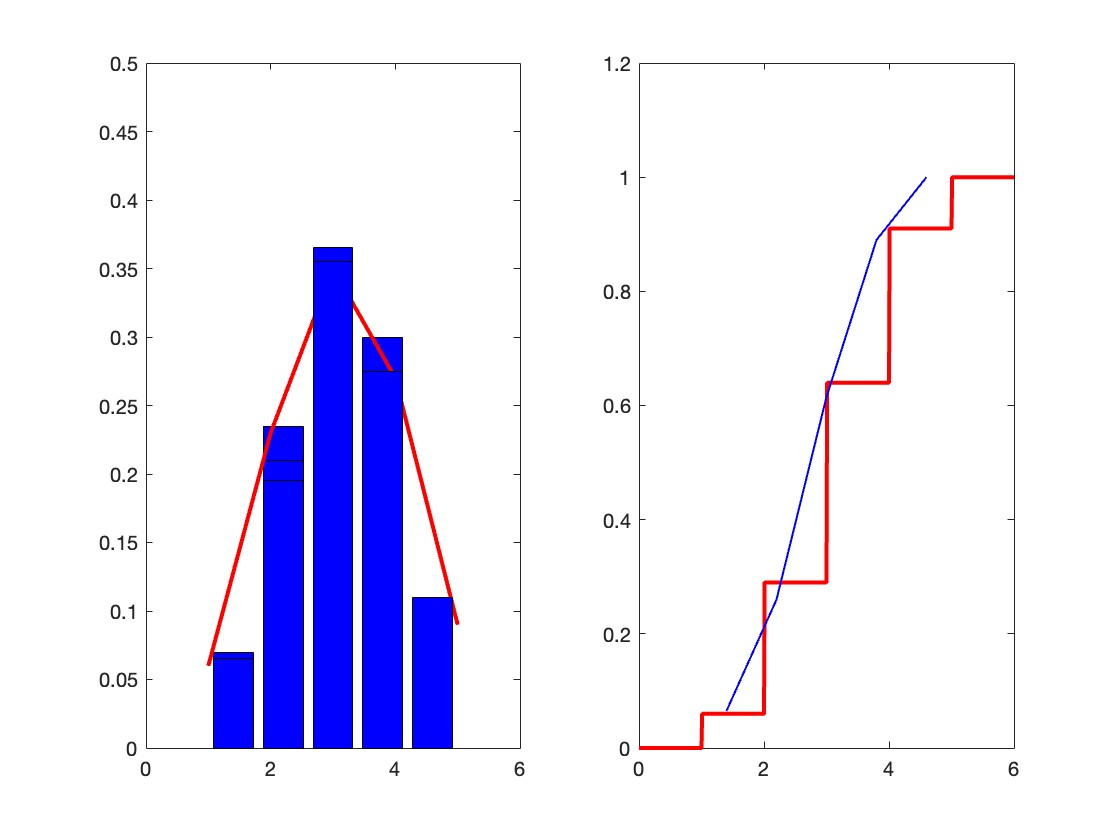
\includegraphics[width=1\linewidth]{../../assets/images/main-content-image.jpg}
    \caption{Hình minh họa 1}
    \label{fig:image1-matlab}
\end{figure}


\begin{matlab}
    \begin{lstlisting}
function Ngocppmohinh(c,j1,j2)
    %UNTITLED Summary of this function goes here
    % Version: 1.0
    %  Date: 10/09/24

    % So tham so
    numpara=j2-j1+1;
    % Dat cac tham so ban dau
    xmin=0; xmax=20; ymin=0; ymax=numpara*4;

    % Import the data
    singletons = readtable("singletons.xlsx");


    % Ve cac doi tuong thanh phan

    for i=1:numpara
    % Ve cac nut tren
    plot((xmin+xmax)/2,ymax-4*(i-1),'ob');
    hold on
    % Ve cac vi tri trang thai
        % tim vi tri cac hang trang thai cua tham so i
        hi=find([singletons{:,2}]==j1+i-1);
        % so trang thai thu i
        ni=length(hi);
        % so gia chia deu chieu ngang x
        dx=(xmax-xmin)/(ni+1);
        % vecto cac diem chia deu chieu ngang x
        x=xmin:dx:xmax;
        % Ve cac duong che ra
        % Vong lap cho tung trang thai
        for t=1:ni
        % Ve cac duong che ra
        plot([x(t+1) (xmin+xmax)/2],[ymax-4*(i-1)-2 ymax-4*(i-1)],'-r');
        hold on
        % Ve cac nut
        plot(x(t+1),ymax-4*(i-1)-2,'ob');
        hold on
        % Chen cac ten trang thai
        text(x(t+1)+.4,ymax-4*(i-1)-2-.4,singletons{hi(t),1});
        % Chen cac duong hoi tu
        plot([x(t+1) (xmin+xmax)/2],[ymax-4*(i-1)-2 ymax-4*(i-1)-4],'-r');
        hold on
        % Chen xac suat
        text(x(t+1)-.9, ymax-4*(i-1)-2+.4, [num2str(singletons{hi(t),5})]);
        end % t=1:ni
    end % for i=1:numpara

        % Ve nut ket thuc
        plot((xmin+xmax)/2,ymin,'ob');
        hold off
        
        % Chen cac 
        title('Graph of the clique Singletons')
        axis([xmin xmax ymin ymax+1])
        
        
        % Ve he truc hoac khong
        if c==0
            axis off
        else
            grid
        end % if c==0
        figure(1)

end % for function
    \end{lstlisting}
\end{matlab}

\begin{dl}
 Nội dung định lý viết vào đây   
\end{dl}

\cm{
Nội dung CM viết vào đây.
}

\begin{tc}
    
\end{tc}

\begin{md}
    
\end{md}

\begin{cy}
    
\end{cy}

\begin{vd}
    
\end{vd}

\begin{nx}
    
\end{nx}

\begin{bd}
    
\end{bd}
\subsection{Tiểu mục 2}
\begin{figure}[h!]
    \centering
    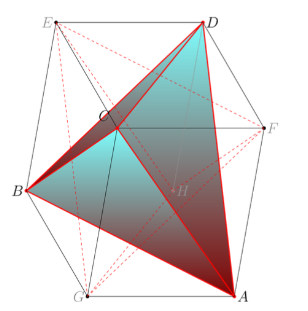
\includegraphics[width=0.3\linewidth]{../../assets/images/figure-1.png}
    \caption{Hình minh họa 1}
    \label{fig:enter-label}
\end{figure}
%%%%%%%%%%%%%%%%%%%%%%%%%%%%%%%%%%%%%%%%%%%%%%%%%%
% nội dung này có thể tham khảo giáo trình ĐSTT và HH2
\section{Mục 2}
\subsection{Tiểu mục 1}

\subsection{Tiểu mục 2}
\chapter{Phân tích nhiều chiều dữ liệu thang đo định lượng}

Phân tích dữ liệu nhiều chiều là một lĩnh vực quan trọng của thống kê hiện đại, cho phép chúng ta khám phá và hiểu mối quan hệ phức tạp giữa nhiều biến số đồng thời \cite{johnson2007, anderson1984, mardia1979}. Chương này sẽ trình bày các kỹ thuật cơ bản và nâng cao trong phân tích nhiều chiều, từ những khái niệm cơ sở đến các ứng dụng thực tiễn.

\section{Khái niệm cơ bản về dữ liệu nhiều chiều}

\subsection{Vector ngẫu nhiên và phân phối nhiều chiều}
\begin{dn}[Vector ngẫu nhiên]
Vector ngẫu nhiên $p$-chiều là một ánh xạ $\mathbf{X}: \Omega \to \mathbb{R}^p$ được viết dưới dạng
\[
\mathbf{X} = \begin{pmatrix} X_1 \\ X_2 \\ \vdots \\ X_p \end{pmatrix}
\]
trong đó mỗi $X_i$ là một biến ngẫu nhiên.
\end{dn}

\subsection{Vector kỳ vọng và ma trận hiệp phương sai}
\begin{dn}[Vector kỳ vọng]
\[
\boldsymbol{\mu} = \mathbb{E}[\mathbf{X}] = \begin{pmatrix} \mathbb{E}[X_1] \\ \mathbb{E}[X_2] \\ \vdots \\ \mathbb{E}[X_p] \end{pmatrix}
\]
\end{dn}

\begin{dn}[Ma trận hiệp phương sai]
\[
\boldsymbol{\Sigma} = \text{Cov}(\mathbf{X}) = \mathbb{E}[(\mathbf{X} - \boldsymbol{\mu})(\mathbf{X} - \boldsymbol{\mu})^T]
\]
với phần tử thứ $(i,j)$ là $\Sigma_{ij} = \text{Cov}(X_i, X_j)$.
\end{dn}

\begin{tinhchat}[Tính chất của ma trận hiệp phương sai]
\begin{itemize}
    \item $\boldsymbol{\Sigma}$ là ma trận đối xứng: $\boldsymbol{\Sigma} = \boldsymbol{\Sigma}^T$
    \item $\boldsymbol{\Sigma}$ là ma trận nửa xác định dương
    \item Đường chéo chính chứa các phương sai: $\Sigma_{ii} = \text{Var}(X_i)$
\end{itemize}
\end{tinhchat}

\subsection{Phân phối chuẩn nhiều chiều}
\begin{dn}[Phân phối chuẩn nhiều chiều]
Vector ngẫu nhiên $\mathbf{X}$ có phân phối chuẩn nhiều chiều $\mathcal{N}_p(\boldsymbol{\mu}, \boldsymbol{\Sigma})$ nếu có hàm mật độ:
\[
f(\mathbf{x}) = \frac{1}{(2\pi)^{p/2}|\boldsymbol{\Sigma}|^{1/2}} \exp\left(-\frac{1}{2}(\mathbf{x} - \boldsymbol{\mu})^T\boldsymbol{\Sigma}^{-1}(\mathbf{x} - \boldsymbol{\mu})\right)
\]
\end{dn}

\section{Ma trận tương quan và các đặc trưng mô tả}

\subsection{Ma trận tương quan}
\begin{dn}[Ma trận tương quan]
Ma trận tương quan $\mathbf{R}$ có phần tử thứ $(i,j)$ là:
\[
\rho_{ij} = \frac{\text{Cov}(X_i, X_j)}{\sqrt{\text{Var}(X_i)\text{Var}(X_j)}} = \frac{\Sigma_{ij}}{\sqrt{\Sigma_{ii}\Sigma_{jj}}}
\]
\end{dn}

Mối quan hệ giữa ma trận hiệp phương sai và ma trận tương quan:
\[
\boldsymbol{\Sigma} = \mathbf{D}^{1/2} \mathbf{R} \mathbf{D}^{1/2}
\]
trong đó $\mathbf{D} = \text{diag}(\Sigma_{11}, \Sigma_{22}, \ldots, \Sigma_{pp})$.

\subsection{Ước lượng mẫu}
Với mẫu $\mathbf{x}_1, \mathbf{x}_2, \ldots, \mathbf{x}_n$:

\textbf{Vector trung bình mẫu:}
\[
\overline{\mathbf{x}} = \frac{1}{n}\sum_{i=1}^n \mathbf{x}_i
\]

\textbf{Ma trận hiệp phương sai mẫu:}
\[
\mathbf{S} = \frac{1}{n-1}\sum_{i=1}^n (\mathbf{x}_i - \overline{\mathbf{x}})(\mathbf{x}_i - \overline{\mathbf{x}})^T
\]

\textbf{Ma trận tương quan mẫu:}
\[
\mathbf{R} = \mathbf{D}_S^{-1/2} \mathbf{S} \mathbf{D}_S^{-1/2}
\]
với $\mathbf{D}_S = \text{diag}(S_{11}, S_{22}, \ldots, S_{pp})$.

\section{Phân tích thành phần chính (Principal Component Analysis - PCA)}

\subsection{Động lực và ý tưởng cơ bản}
PCA là kỹ thuật giảm chiều dữ liệu bằng cách tìm các hướng có phương sai lớn nhất. Mục tiêu là chuyển đổi dữ liệu gốc $p$-chiều thành không gian mới có chiều thấp hơn mà vẫn giữ được nhiều thông tin nhất.

\subsection{Định nghĩa toán học}
\begin{dn}[Thành phần chính thứ nhất]
Thành phần chính thứ nhất là tổ hợp tuyến tính $Y_1 = \mathbf{a}_1^T\mathbf{X}$ sao cho:
\begin{itemize}
    \item $\text{Var}(Y_1) = \mathbf{a}_1^T\boldsymbol{\Sigma}\mathbf{a}_1$ đạt giá trị lớn nhất
    \item Ràng buộc: $\|\mathbf{a}_1\| = 1$
\end{itemize}
\end{dn}

\begin{dl}[Nghiệm của bài toán PCA]
Các thành phần chính được xác định thông qua phân tích trị riêng của ma trận hiệp phương sai:
\[
\boldsymbol{\Sigma}\mathbf{a}_i = \lambda_i\mathbf{a}_i, \quad i = 1, 2, \ldots, p
\]
với $\lambda_1 \geq \lambda_2 \geq \cdots \geq \lambda_p \geq 0$ và $\|\mathbf{a}_i\| = 1$.
\end{dl}

\subsection{Tính chất quan trọng}
\begin{tinhchat}[Tính chất của PCA]
\begin{itemize}
    \item Phương sai của thành phần chính thứ $i$: $\text{Var}(Y_i) = \lambda_i$
    \item Tổng phương sai được bảo toàn: $\sum_{i=1}^p \lambda_i = \sum_{i=1}^p \text{Var}(X_i)$
    \item Các thành phần chính không tương quan: $\text{Cov}(Y_i, Y_j) = 0$ với $i \neq j$
    \item Tỷ lệ phương sai được giải thích bởi $k$ thành phần đầu: $\frac{\sum_{i=1}^k \lambda_i}{\sum_{i=1}^p \lambda_i}$
\end{itemize}
\end{tinhchat}

\subsection{Thuật toán thực hiện PCA}
\begin{enumerate}
    \item \textbf{Chuẩn hóa dữ liệu}: Chuyển về dạng $Z$-score nếu cần
    \item \textbf{Tính ma trận hiệp phương sai} (hoặc tương quan)
    \item \textbf{Phân tích trị riêng}: Tìm $\lambda_i$ và $\mathbf{a}_i$
    \item \textbf{Sắp xếp}: Theo thứ tự giảm dần của $\lambda_i$
    \item \textbf{Chọn số thành phần}: Dựa trên tiêu chí phù hợp
    \item \textbf{Chuyển đổi dữ liệu}: $\mathbf{Y} = \mathbf{A}^T\mathbf{X}$
\end{enumerate}

\subsection{Tiêu chí lựa chọn số thành phần}
\subsubsection*{Tiêu chí Kaiser}
Giữ lại các thành phần có $\lambda_i > 1$ (khi sử dụng ma trận tương quan).

\subsubsection*{Tiêu chí phần trăm phương sai}
Chọn $k$ sao cho $\frac{\sum_{i=1}^k \lambda_i}{\sum_{i=1}^p \lambda_i} \geq 0.80$ (hoặc 0.85, 0.90).

\subsubsection*{Scree plot}
Vẽ đồ thị $\lambda_i$ theo $i$ và tìm "điểm khuỷu" (elbow point).

\section{Phân tích nhân tố (Factor Analysis)}

\subsection{Mô hình nhân tố}
\begin{dn}[Mô hình nhân tố]
Mô hình nhân tố biểu diễn vector quan sát $\mathbf{X}$ dưới dạng:
\[
\mathbf{X} = \boldsymbol{\mu} + \mathbf{L}\mathbf{F} + \boldsymbol{\epsilon}
\]
trong đó:
\begin{itemize}
    \item $\mathbf{F}$ là vector nhân tố chung $(m \times 1)$ với $m < p$
    \item $\mathbf{L}$ là ma trận tải nhân tố $(p \times m)$
    \item $\boldsymbol{\epsilon}$ là vector sai số cụ thể $(p \times 1)$
\end{itemize}
\end{dn}

\subsection{Giả định của mô hình}
\begin{itemize}
    \item $\mathbb{E}[\mathbf{F}] = \mathbf{0}$ và $\text{Cov}(\mathbf{F}) = \mathbf{I}_m$
    \item $\mathbb{E}[\boldsymbol{\epsilon}] = \mathbf{0}$ và $\text{Cov}(\boldsymbol{\epsilon}) = \boldsymbol{\Psi}$ (ma trận chéo)
    \item $\text{Cov}(\mathbf{F}, \boldsymbol{\epsilon}) = \mathbf{0}$
\end{itemize}

\subsection{Phân tích ma trận hiệp phương sai}
Từ mô hình nhân tố, ta có:
\[
\boldsymbol{\Sigma} = \mathbf{L}\mathbf{L}^T + \boldsymbol{\Psi}
\]

\textbf{Phương sai chung (communality):} $h_i^2 = \sum_{j=1}^m L_{ij}^2$

\textbf{Phương sai cụ thể (specific variance):} $\psi_i = \Sigma_{ii} - h_i^2$

\subsection{Phương pháp ước lượng}
\subsubsection*{Phương pháp thành phần chính}
Sử dụng $m$ thành phần chính đầu tiên để ước lượng ma trận tải:
\[
\hat{\mathbf{L}} = \mathbf{A}_m\boldsymbol{\Lambda}_m^{1/2}
\]
với $\mathbf{A}_m$ chứa $m$ vector riêng đầu và $\boldsymbol{\Lambda}_m = \text{diag}(\lambda_1, \ldots, \lambda_m)$.

\subsubsection*{Phương pháp maximum likelihood}
Tối đa hóa hàm likelihood dưới giả định phân phối chuẩn.

\subsection{Xoay nhân tố (Factor Rotation)}
Mục đích: Tìm ma trận tải dễ giải thích hơn thông qua phép xoay.

\subsubsection*{Xoay Varimax}
Tối đa hóa tổng phương sai của bình phương các tải trong mỗi nhân tố:
\[
V = \sum_{j=1}^m \left[\sum_{i=1}^p L_{ij}^4 - \frac{1}{p}\left(\sum_{i=1}^p L_{ij}^2\right)^2\right]
\]

\subsubsection*{Xoay Promax}
Cho phép các nhân tố tương quan với nhau (oblique rotation).

\section{Áp dụng thuật toán trên R}

Bộ dữ liệu nghiên cứu được thu thập thông qua phiếu khảo sát dành cho giảng viên, chuyên viên, học viên cao học và sinh viên Trường Đại học Cần Thơ, nhằm đánh giá toàn diện mức độ cần thiết, hiệu quả, sự hài lòng và mức độ quan tâm đối với các hoạt động dịch vụ thông tin thư viện tại Trung tâm Học liệu. Phiếu khảo sát bao gồm nhiều nhóm tiêu chí liên quan đến:
\begin{itemize}
    \item Mục đích và vai trò của hoạt động dịch vụ thông tin thư viện.
    \item Các phương pháp triển khai hoạt động dịch vụ.
    \item Mức độ hài lòng và tần suất sử dụng các loại hình dịch vụ.
    \item Mức độ quan tâm của các nhóm đối tượng thụ hưởng.
    \item Điều kiện cơ sở vật chất, hạ tầng và hỗ trợ thông tin.
    \item Tầm quan trọng của công tác quản lý dịch vụ.
\end{itemize}

Các câu hỏi được xây dựng theo thang đo Likert nhiều mức, từ ``Rất cần thiết'' đến ``Không cần thiết'' hoặc từ ``Rất hài lòng'' đến ``Rất không hài lòng'', cho phép định lượng thái độ và nhận thức của người trả lời.

Bộ dữ liệu sau khi thu thập, xử lý được lưu lại với dạng bảng hỏi gồm 60 biến trong excel. Bên dưới minh họa một vài biến trong dữ liệu như sau:
\begin{figure}[h!]
    \centering
    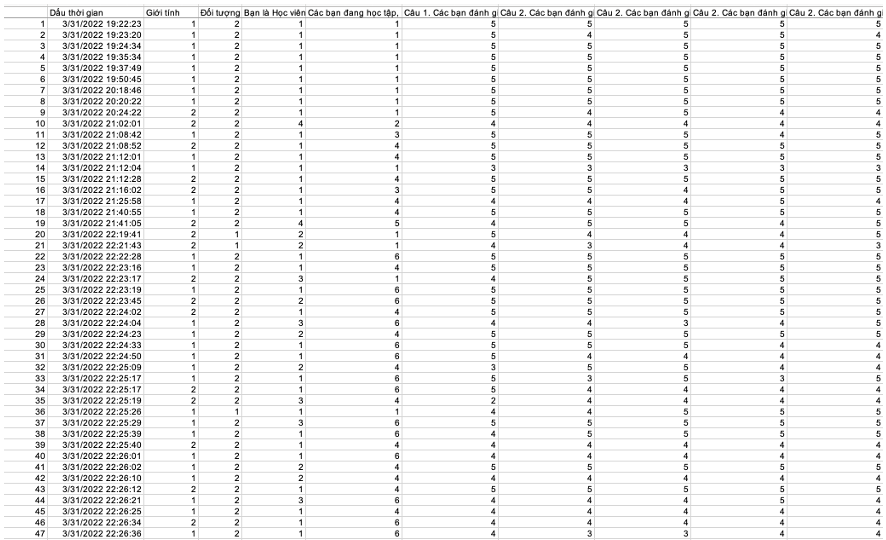
\includegraphics[width=\textwidth]{../../assets/images/SP19.png}
    \caption{Minh họa dữ liệu gốc với 60 biến}
    \label{fig:original_data}
\end{figure}

Với bộ dữ liệu này, tiến hành xáo trộn. Khi đó, chúng tôi thu được dữ liệu khác với cấu trúc ban đầu như sau:
\begin{figure}[h!]
    \centering
    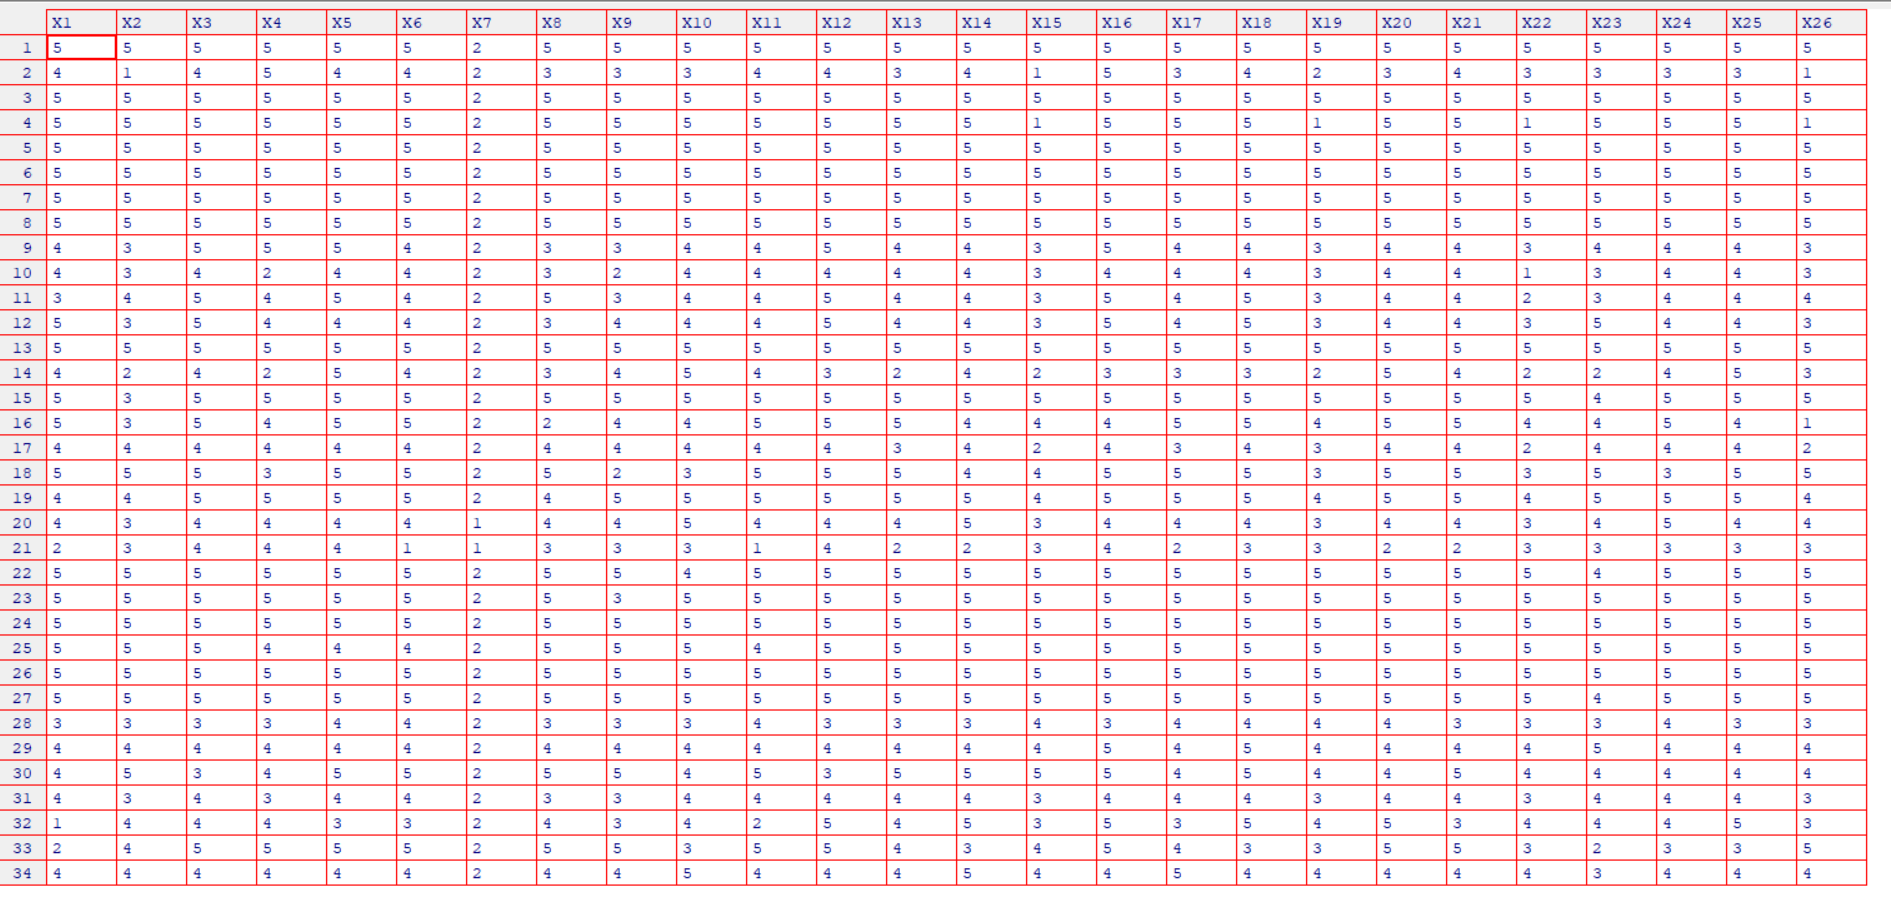
\includegraphics[width=\textwidth]{../../assets/images/data2b.png}
    \caption{Dữ liệu sau khi xáo trộn}
    \label{fig:shuffled_data}
\end{figure}

Để khám phá và xác định cấu trúc tiềm ẩn của dữ liệu, quy trình phân tích được triển khai theo hai bước:

\begin{enumerate}
    \item \textbf{Phân tích thành phần chính (Principal Component Analysis -- PCA)}:
    \begin{itemize}
        \item Xác định số lượng thành phần chính có khả năng giải thích phần lớn phương sai của dữ liệu.
        \item Đánh giá mức độ tương quan giữa các biến quan sát và loại bỏ các biến có tải số thấp hoặc không đạt yêu cầu.
        \item Sử dụng kết quả biểu đồ Scree Plot và giá trị Eigenvalue để đề xuất số nhân tố tiềm năng cho bước EFA.
    \end{itemize}

    \item \textbf{Phân tích nhân tố khám phá (Exploratory Factor Analysis -- EFA)}:
    \begin{itemize}
        \item Xác nhận và nhóm các biến quan sát thành các nhân tố đại diện.
        \item Kiểm định độ tin cậy và tính hội tụ của các thang đo.
        \item Loại bỏ các biến có hệ số tải nhân tố thấp hoặc tải chéo cao.
    \end{itemize}
\end{enumerate}

Cách tiếp cận này đảm bảo quá trình trích xuất nhân tố được thực hiện có cơ sở thống kê vững chắc, đồng thời tối ưu hóa khả năng giải thích và ứng dụng của mô hình nghiên cứu, phục vụ cho các bước phân tích suy luận và đề xuất giải pháp nâng cao chất lượng dịch vụ thông tin thư viện.

\subsection*{Bắt đầu quy trình phân tích:}
\textbf{1. Phân tích thành phần chính (PCA):} 

\text{Đọc dữ liệu vào R và xử lý dữ liệu ban đầu để tiến hành phân tích với code sau:}
\begin{lstlisting}[style=Rstyle, caption={Đọc dữ liệu vào để tiến hành phân tích dữ liệu}]
# INSTALL AND LOAD REQUIRED PACKAGES
# List of required packages with specific versions (if needed)
packages <- c("psych", "GPArotation", "ggplot2", "corrplot", "factoextra", 
             "nFactors", "dplyr", "knitr", "kableExtra", "rmarkdown")

# Install only missing packages
installed <- rownames(installed.packages())
to_install <- setdiff(packages, installed)
if(length(to_install) > 0) install.packages(to_install)

# Load libraries with error handling
suppressPackageStartupMessages({
  library(psych)        # For factor analysis and reliability tests
  library(GPArotation)  # For factor rotation methods
  library(ggplot2)      # For advanced visualizations
  library(corrplot)     # For correlation matrix visualization
  library(factoextra)   # For PCA visualization
  library(nFactors)     # For determining number of factors
  library(dplyr)        # For data manipulation
  library(knitr)        # For reporting
  library(kableExtra)   # For nice tables
})

# DATA IMPORT AND PREPROCESSING ================================================

# Read data from CSV file with error handling
tryCatch({
  setwd("D:/09_ThayLy/Chuyen_de_thong_ke_nang_cao/EFA")
  data <- read.csv("Data2b.csv", header = TRUE, stringsAsFactors = FALSE)
}, error = function(e) {
  stop("Error reading data file. Please check file path and format.")
})

# Initial data inspection
cat("\n=== DATA STRUCTURE ===\n")
str(data)
cat("\nFirst 5 rows:\n")
print(head(data, 5))

# Check for missing values
missing_values <- sum(is.na(data))
if(missing_values > 0) {
  cat("\nWarning:", missing_values, "missing values found.\n")
  # Visualize missing values
  if(require(visdat)) {
    visdat::vis_miss(data)
  }
} else {
  cat("\nNo missing values found.\n")
}

# Handle missing values by listwise deletion
data_clean <- na.omit(data)
cat("\nOriginal data:", nrow(data), "rows")
cat("\nAfter removing NAs:", nrow(data_clean), "rows")

# Check for zero variance variables
zero_var <- sapply(data_clean, function(x) var(x, na.rm = TRUE) == 0)
if(any(zero_var)) {
  cat("\nWarning: Zero variance variables detected:", names(data_clean)[zero_var], "\n")
  data_clean <- data_clean[, !zero_var]
}
\end{lstlisting}

\text{Sau đó, tiến hành kiểm định tương quan giữa các biến:}
\begin{lstlisting}[caption={Phân tích tương quan giữa các biến}]
# CORRELATION ANALYSIS ========================================================

# Calculate correlation matrix with handling for non-numeric columns
cor_matrix <- cor(data_clean[, sapply(data_clean, is.numeric)])

# Create publication-ready correlation plot
corr_plot <- function(cor_matrix) {
  corrplot(cor_matrix, 
           method = "color", 
           type = "upper",
           order = "hclust",
           tl.col = "black", 
           tl.srt = 45,
           tl.cex = 0.7,
           addCoef.col = "black",
           number.cex = 0.5,
           diag = FALSE,
           col = colorRampPalette(c("#BB4444", "#EE9988", "#FFFFFF", "#77AADD", "#4477AA"))(200),
           mar = c(0, 0, 1, 0))
 }

# Save correlation plot to file
png("correlation_matrix.png", width = 14, height = 12, units = "in", res = 300)
corr_plot(cor_matrix)
dev.off()
\end{lstlisting}

Kết quả kiểm định được minh họa bởi ma trận tương quan sau:
\begin{figure}[h!]
    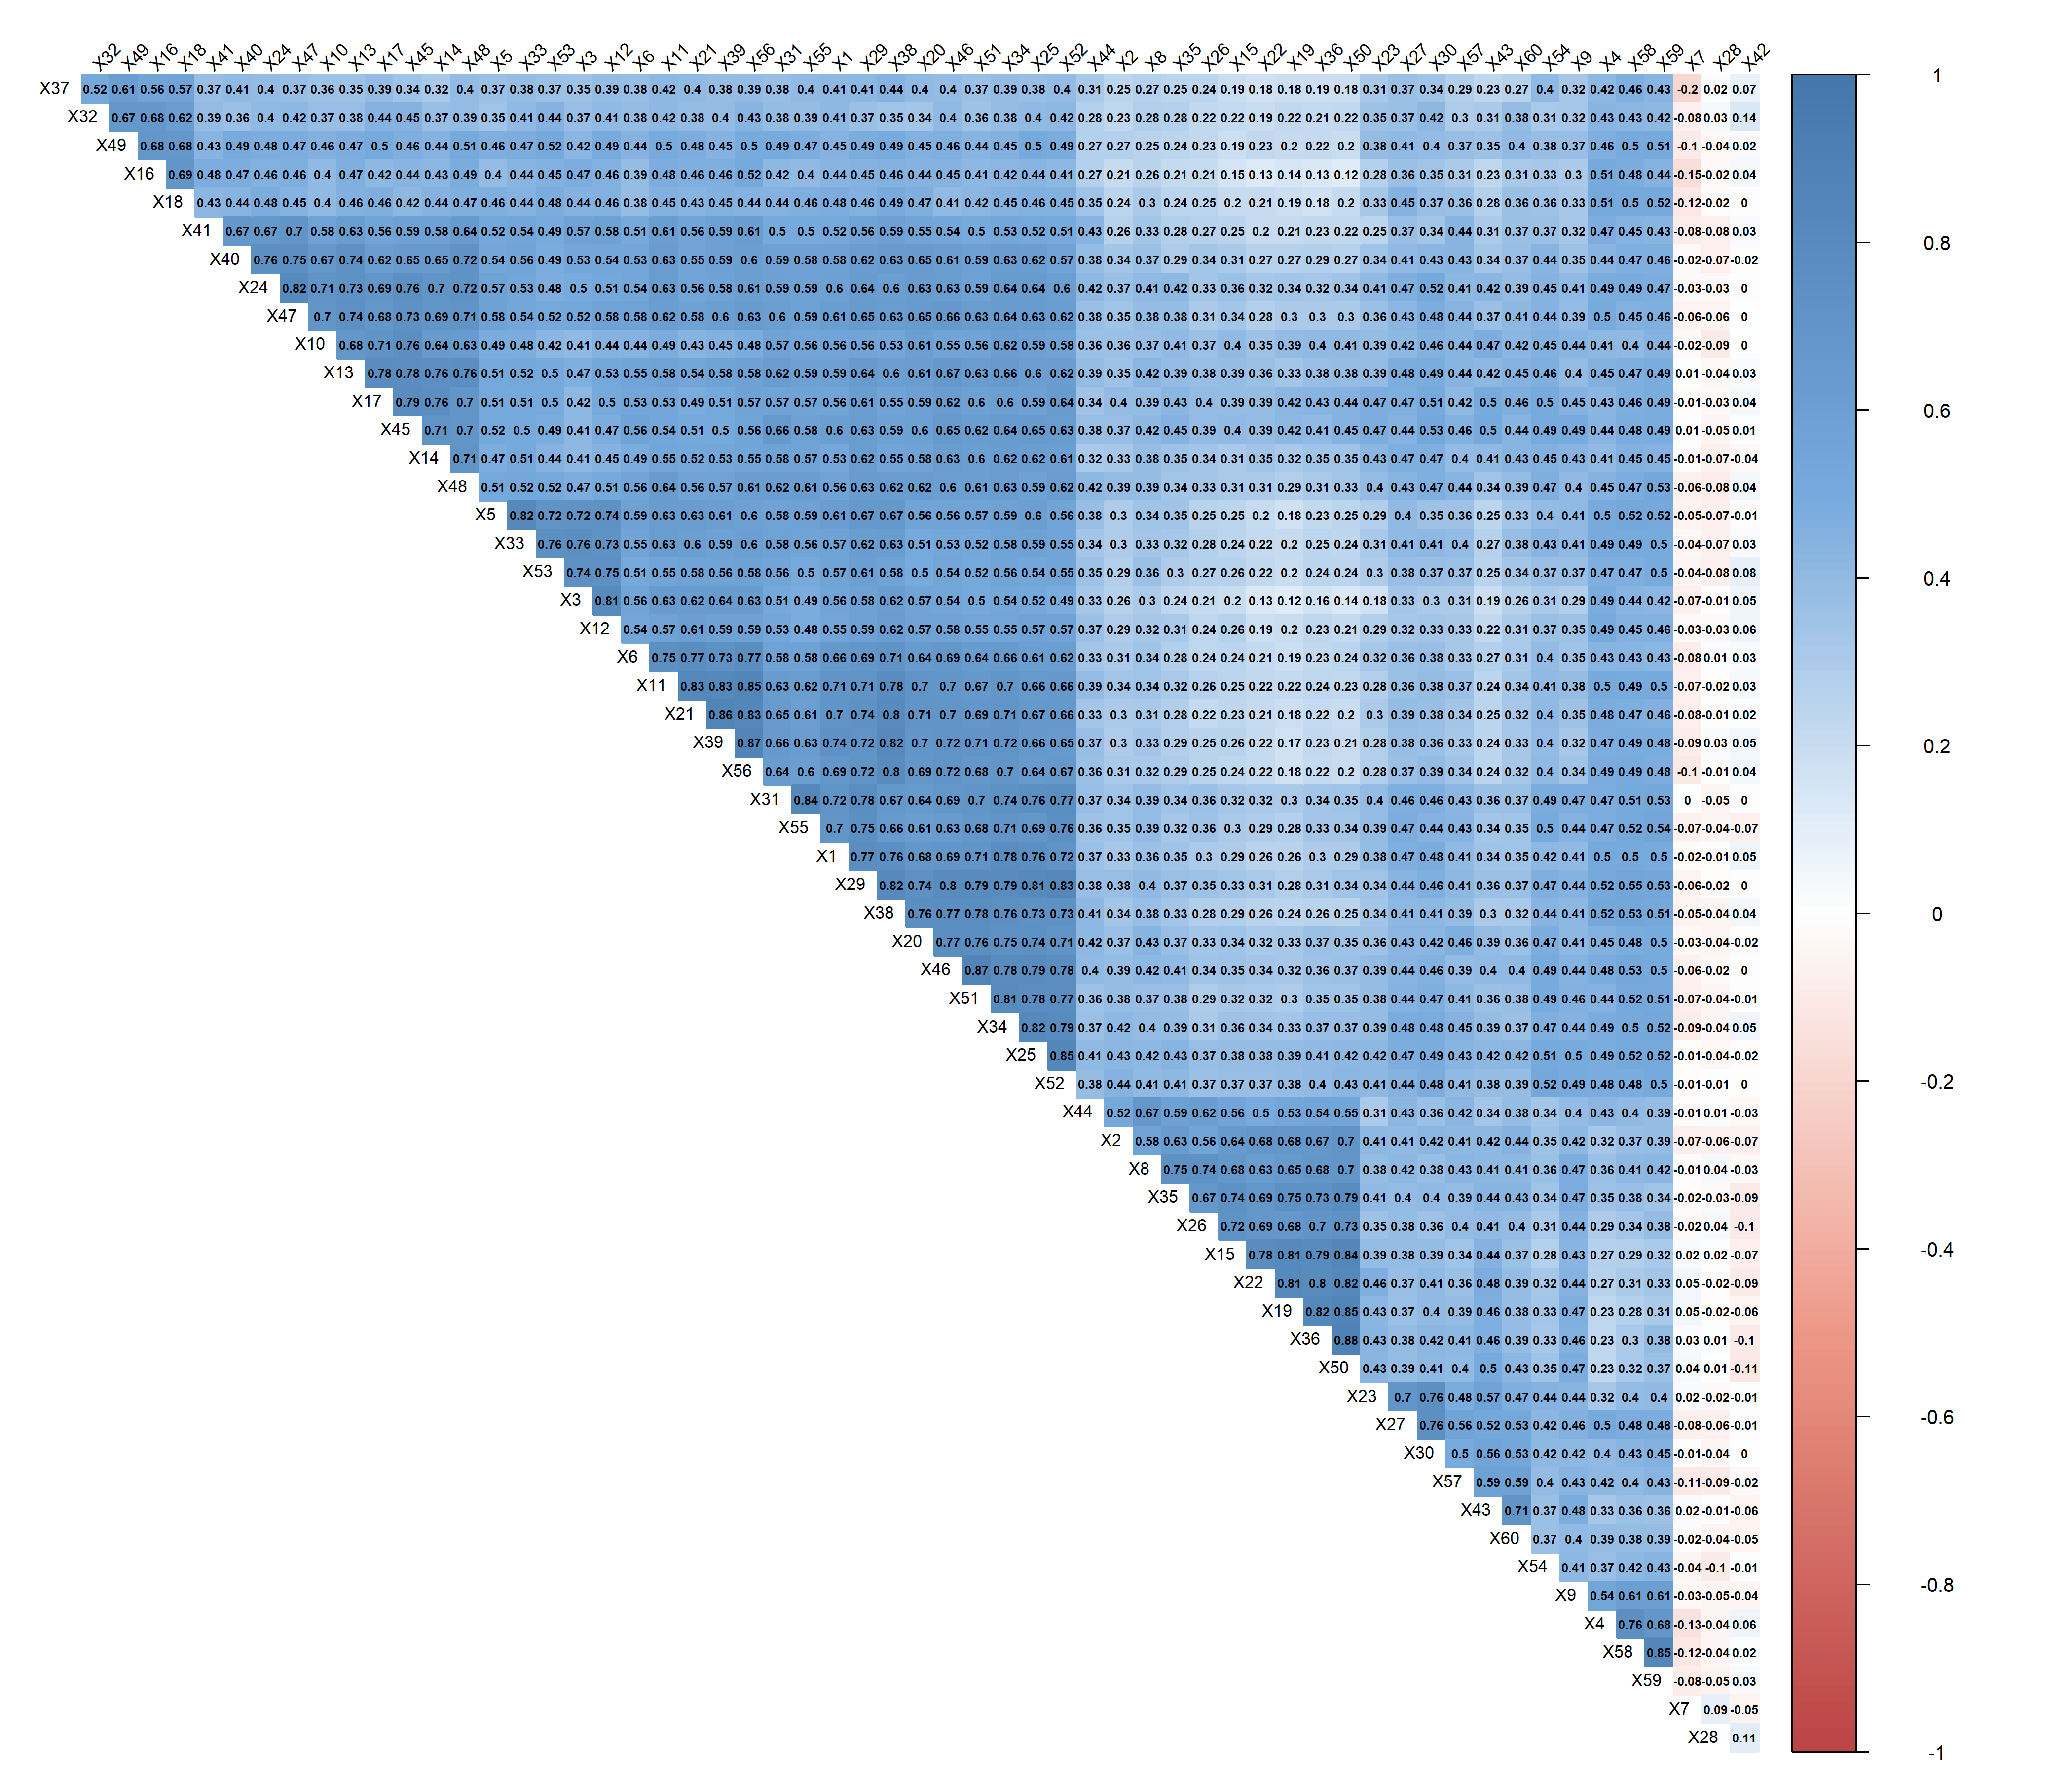
\includegraphics[width=\textwidth]{../../assets/images/correlation_matrix_1.png}
    \caption{Ma trận tương quan giữa các biến}
    \label{fig:correlation_matrix}
\end{figure}

\textbf{Đánh giá độ phù hợp của dữ liệu trước khi phân tích:}
\begin{itemize}
    \item Kiểm định Kaiser-Meyer-Olkin (KMO):
    \begin{lstlisting}
# ASSUMPTION CHECKS FOR FACTOR ANALYSIS =======================================

# Kaiser-Meyer-Olkin (KMO) Measure of Sampling Adequacy
kmo_check <- function(data) {
  kmo_result <- KMO(data)
  cat("\n=== KMO TEST RESULTS ===\n")
  print(kmo_result)
  
  # Interpretation
  kmo_overall <- kmo_result$MSA
  cat("\nKMO Overall:", kmo_overall, "\n")
  if(kmo_overall >= 0.90) {
    cat("Interpretation: Marvelous\n")
  } else if(kmo_overall >= 0.80) {
    cat("Interpretation: Meritorious\n")
  } else if(kmo_overall >= 0.70) {
    cat("Interpretation: Middling\n")
  } else if(kmo_overall >= 0.60) {
    cat("Interpretation: Mediocre\n")
  } else {
    cat("Interpretation: Unacceptable\n")
  }
  
  # Identify problematic variables (MSA < 0.5)
  bad_vars <- names(which(kmo_result$MSAi < 0.5))
  if(length(bad_vars) > 0) {
    cat("\nVariables with KMO < 0.5 (consider removing):\n")
    print(bad_vars)
  }
  
  return(kmo_result)
}

kmo_result <- kmo_check(data_clean)
    \end{lstlisting}
    
    Kết quả cho thấy KMO = 0.97, đạt mức "Marvelous" cho thấy dữ liệu rất phù hợp để tiến hành phân tích nhân tố.

\item Kiểm định Bartlett's Test
    \begin{lstlisting}[caption={Code kiểm định Bartlett's Test}]
# Bartlett's Test of Sphericity
bartlett_check <- function(data) {
  result <- cortest.bartlett(data)
  
  cat("\n=== BARTLETT'S TEST ===\n")
  cat("Chi-square:", round(result$chisq, 2), "\n")
  cat("p-value:", ifelse(result$p.value < 0.001, "< 0.001", round(result$p.value, 4)), "\n")
  
  if(result$p.value < 0.05) {
    cat("Result: Significant (data suitable for factor analysis)\n")
  } else {
    cat("Result: Not significant (data may not be suitable)\n")
  }
  
  return(result)
}

bartlett_result <- bartlett_check(data_clean)
    \end{lstlisting}
\end{itemize}

Tiến hành kiểm định PCA, với chương trình code như sau:
\begin{lstlisting}
# PRINCIPAL COMPONENT ANALYSIS (PCA) ==========================================

# Enhanced PCA function with automatic reporting
run_pca <- function(data, scale = TRUE) {
  pca_result <- prcomp(data, scale. = scale)
  
  # Variance explained
  variance <- pca_result$sdev^2
  prop_var <- variance / sum(variance)
  cum_var <- cumsum(prop_var)
  
  # Create summary table
  pca_summary <- data.frame(
    Component = 1:length(pca_result$sdev),
    Eigenvalue = variance,
    Proportion = prop_var,
    Cumulative = cum_var
  )
  
  cat("\n=== PCA SUMMARY ===\n")
  print(pca_summary)
  
  # Determine number of components
  n_components <- sum(variance > 1) # Kaiser's rule
  cat("\nNumber of components with eigenvalue > 1:", n_components, "\n")
  
  return(list(
    pca = pca_result,
    summary = pca_summary,
    n_components = n_components
  ))
}

pca_results <- run_pca(data_clean)
\end{lstlisting}

Kết quả cho thấy 10 thành phần chính đầu tiên giải thích được 75.80\% tổng phương sai, với thành phần đầu tiên giải thích 45.70\% phương sai.

\begin{figure}[h!]
    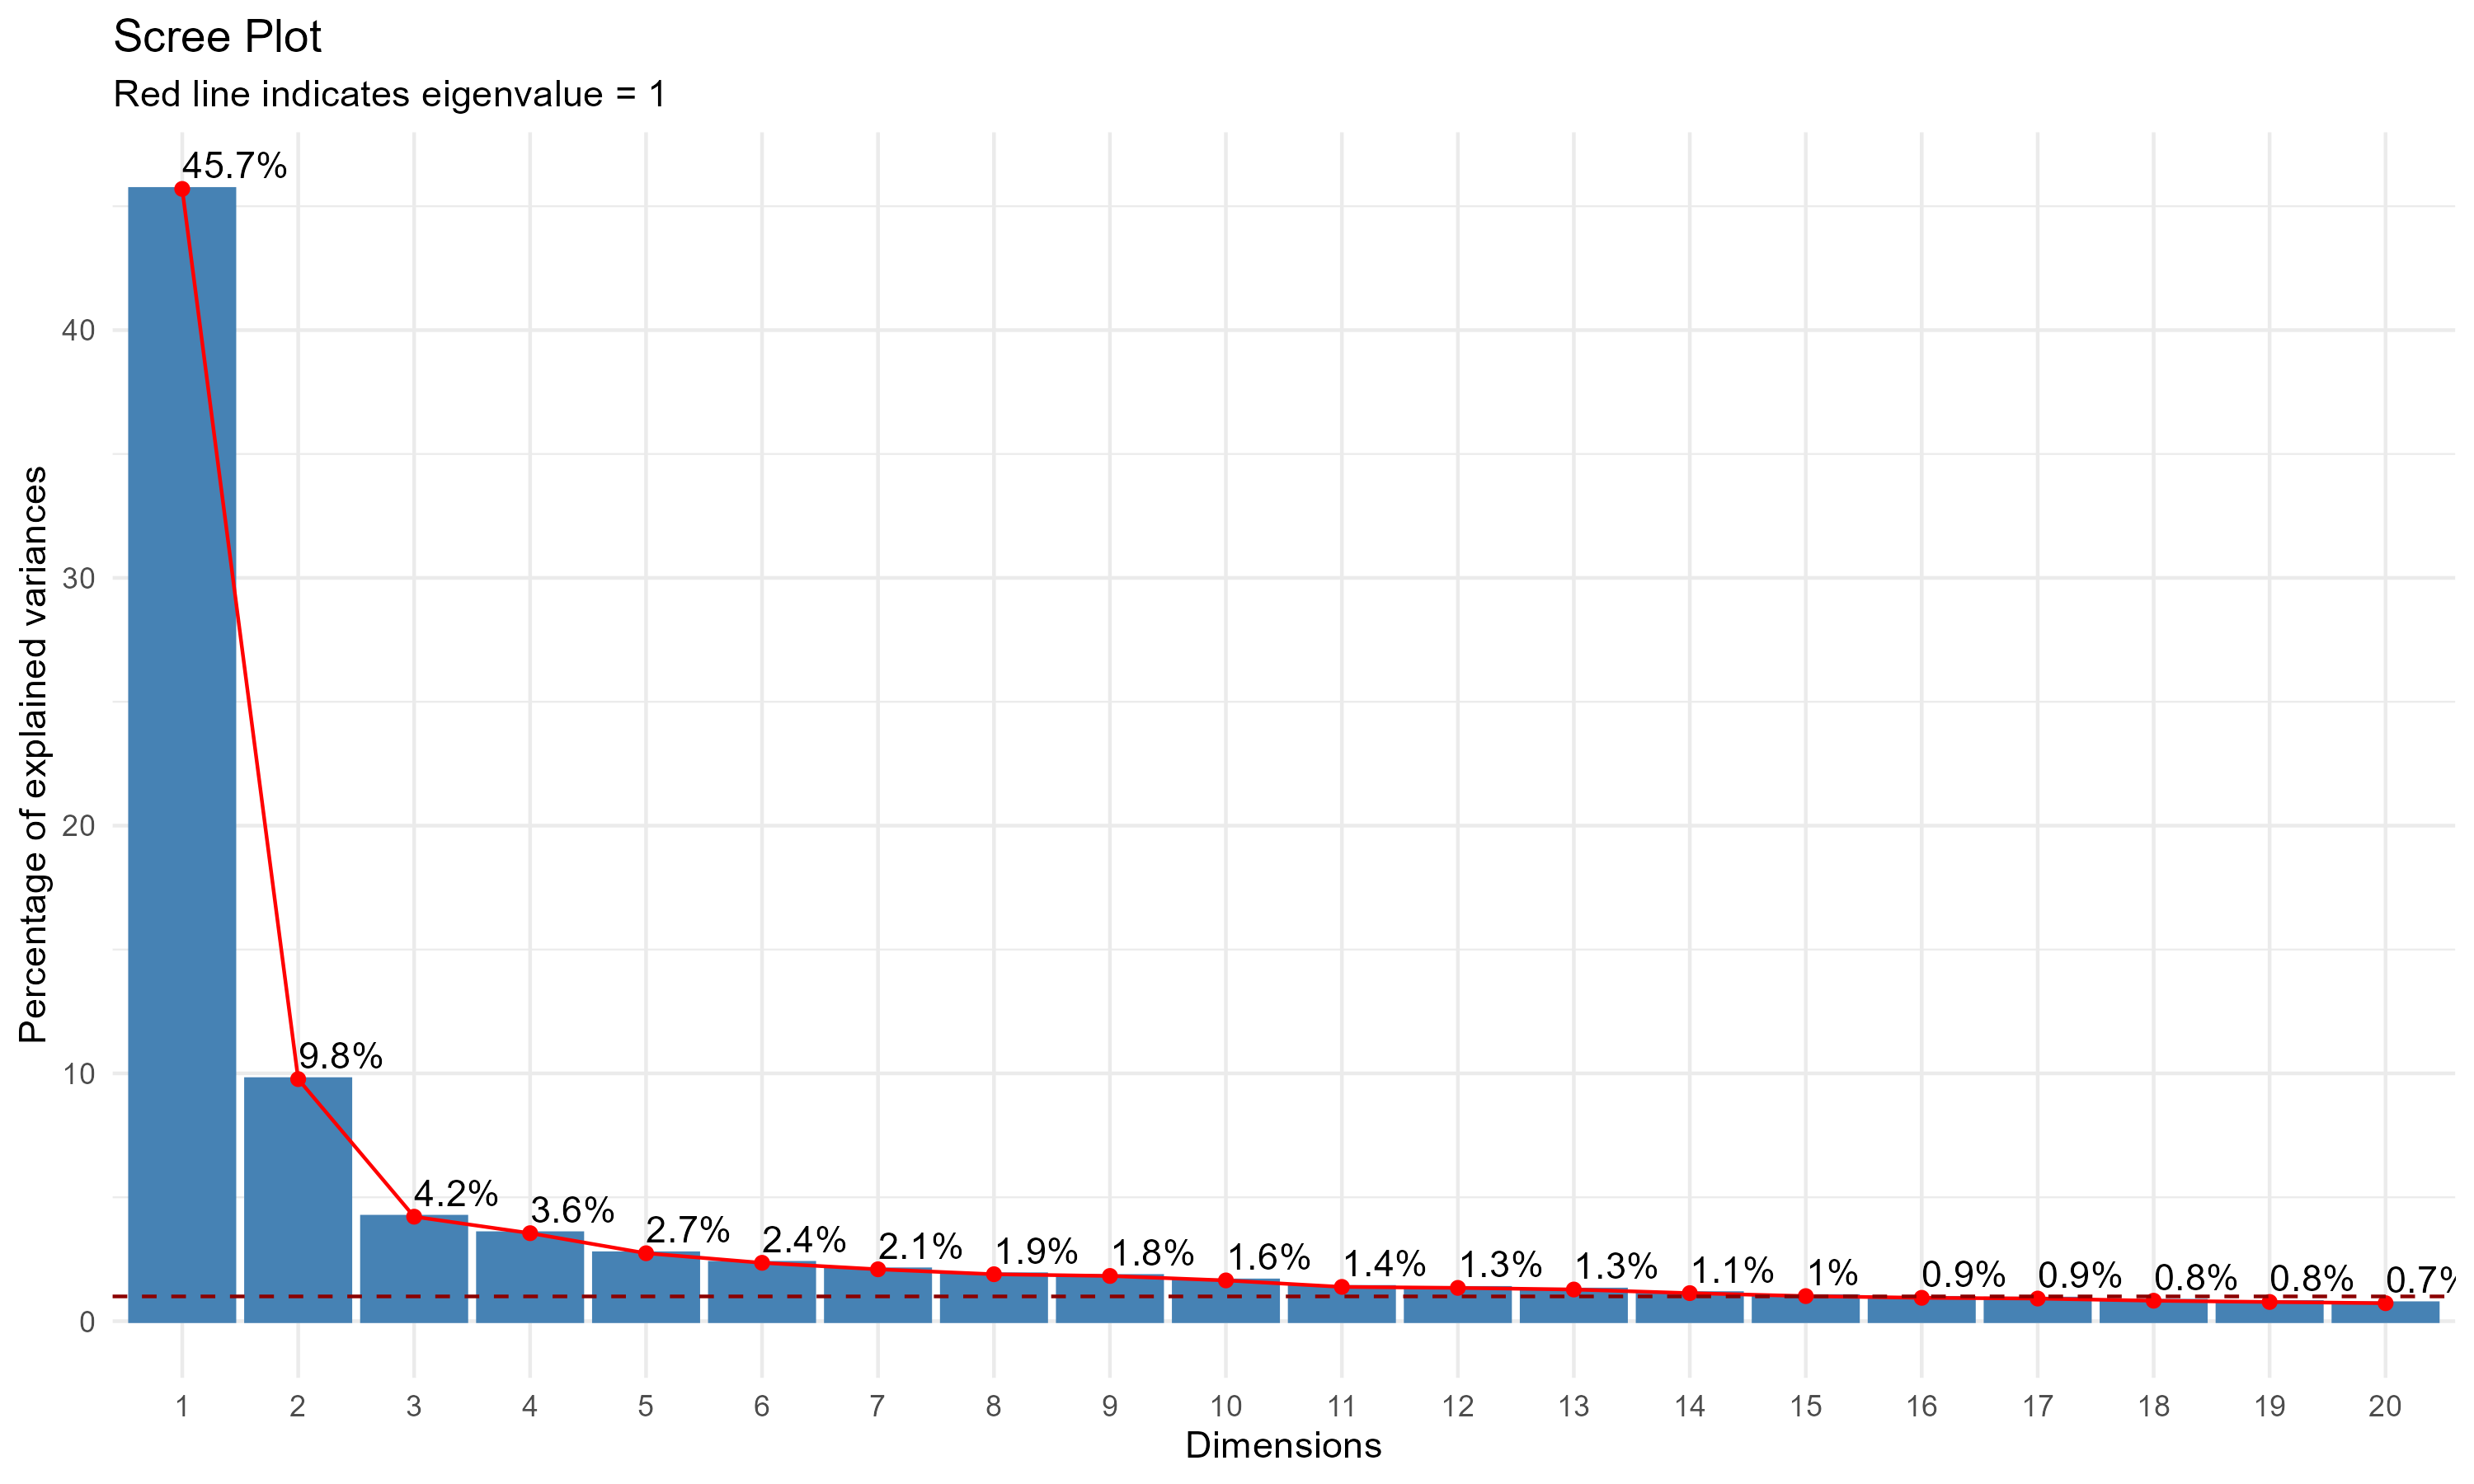
\includegraphics[width=\textwidth]{../../assets/images/SP42.png}
    \caption{Minh họa thành phần phương sai đóng góp}
    \label{fig:scree_plot}
\end{figure}

\begin{figure}[h!]
    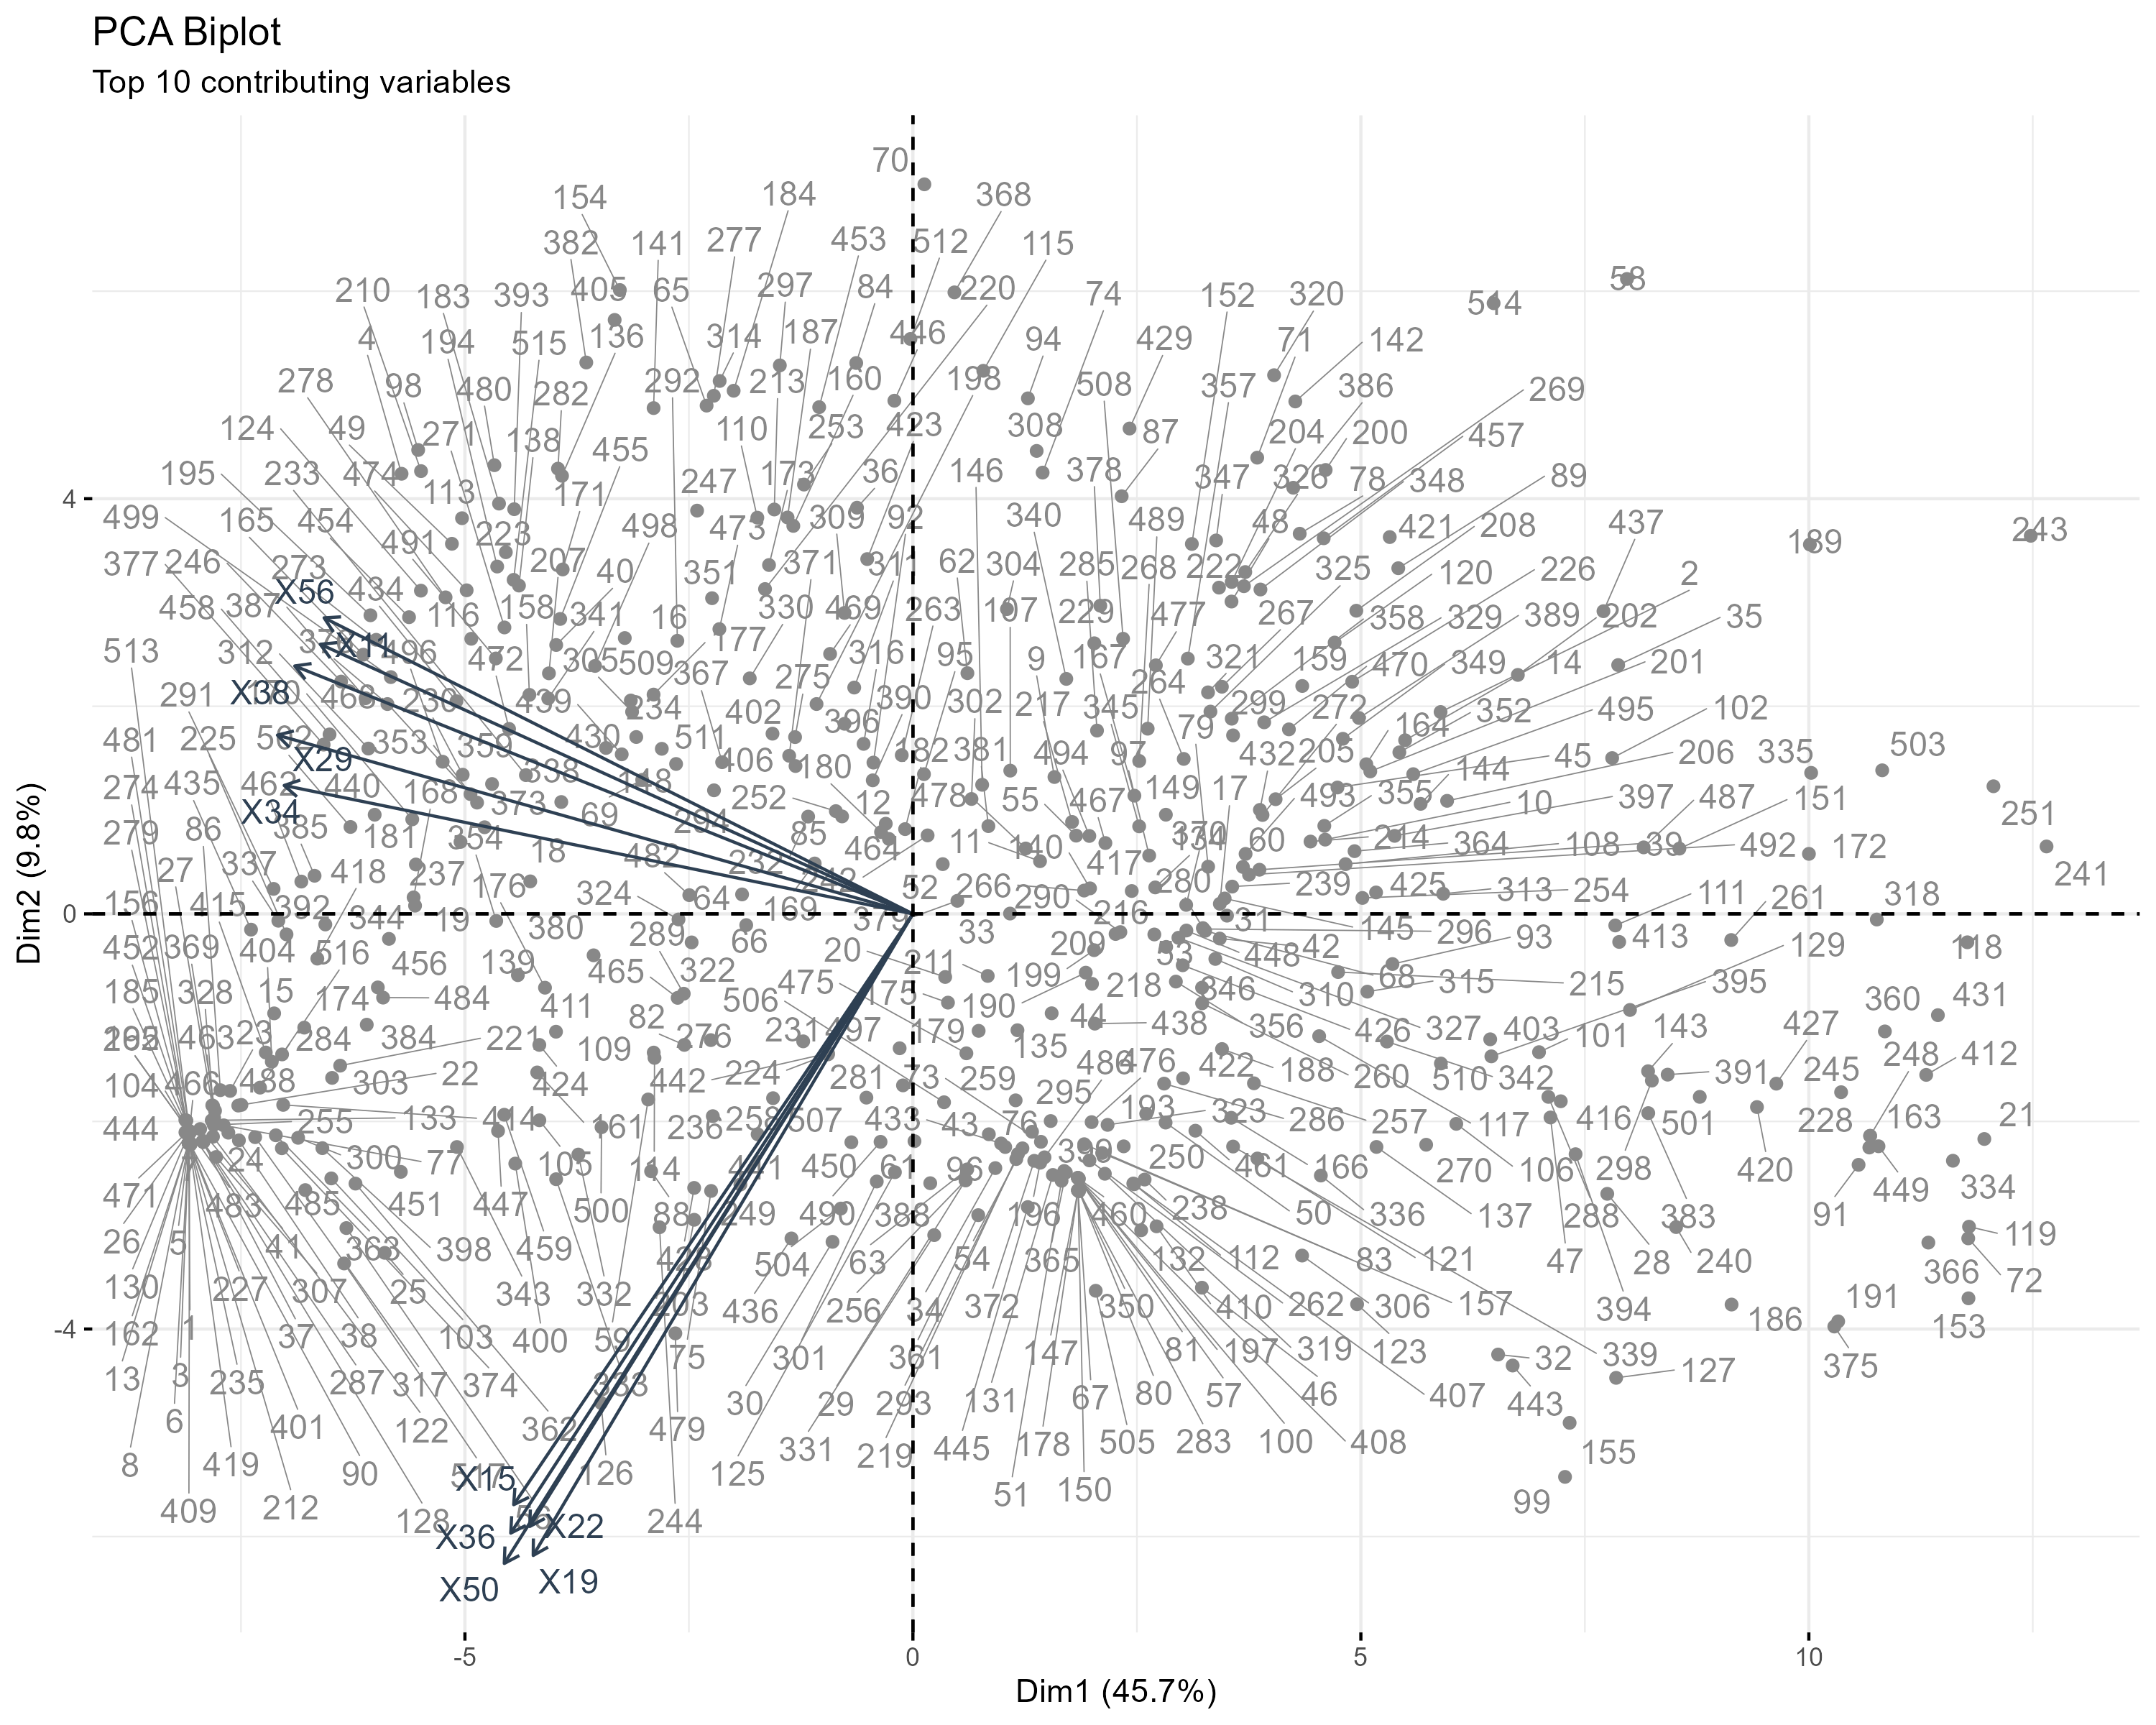
\includegraphics[width=0.9\textwidth]{../../assets/images/SP43.png}
    \caption{Top 10 các biến đóng góp}
    \label{fig:contributions}
\end{figure}

\subsection{Bước 5: Phân tích nhân tố khám phá (EFA)}

Với dữ liệu trên, tiếp tục phân tích nhân tố khám phá (EFA) với chương trinh R như sau:

\begin{lstlisting}
# EXPLORATORY FACTOR ANALYSIS (EFA) ===========================================

# Enhanced EFA function with rotation options and diagnostics
run_efa <- function(data, nfactors = NULL, rotate = "varimax", fm = "ml") {
  
  # Determine number of factors if not specified
  if(is.null(nfactors)) {
    cat("\nDetermining optimal number of factors...\n")
    parallel <- fa.parallel(data, 
                          fa = "fa",
                          n.iter = 100,
                          plot = FALSE)
    nfactors <- parallel$nfact
    cat("Suggested number of factors:", nfactors, "\n")
  }
  
  # Run EFA
  efa_result <- fa(data, 
                  nfactors = nfactors,
                  rotate = rotate,
                  fm = fm,
                  scores = "regression")
  
  # Print loadings with nice formatting
  cat("\n=== FACTOR LOADINGS ===\n")
  print(efa_result$loadings, cutoff = 0.4, sort = TRUE)
  
  return(list(
    efa = efa_result,
    nfactors = nfactors
  ))
}

# Run EFA analysis
efa_results <- run_efa(data_clean)
\end{lstlisting}

Kết quả phân tích EFA cho thấy 8 nhân tố được trích xuất, giải thích được 68.2\% tổng phương sai:

\begin{figure}[h!]
    \centering
        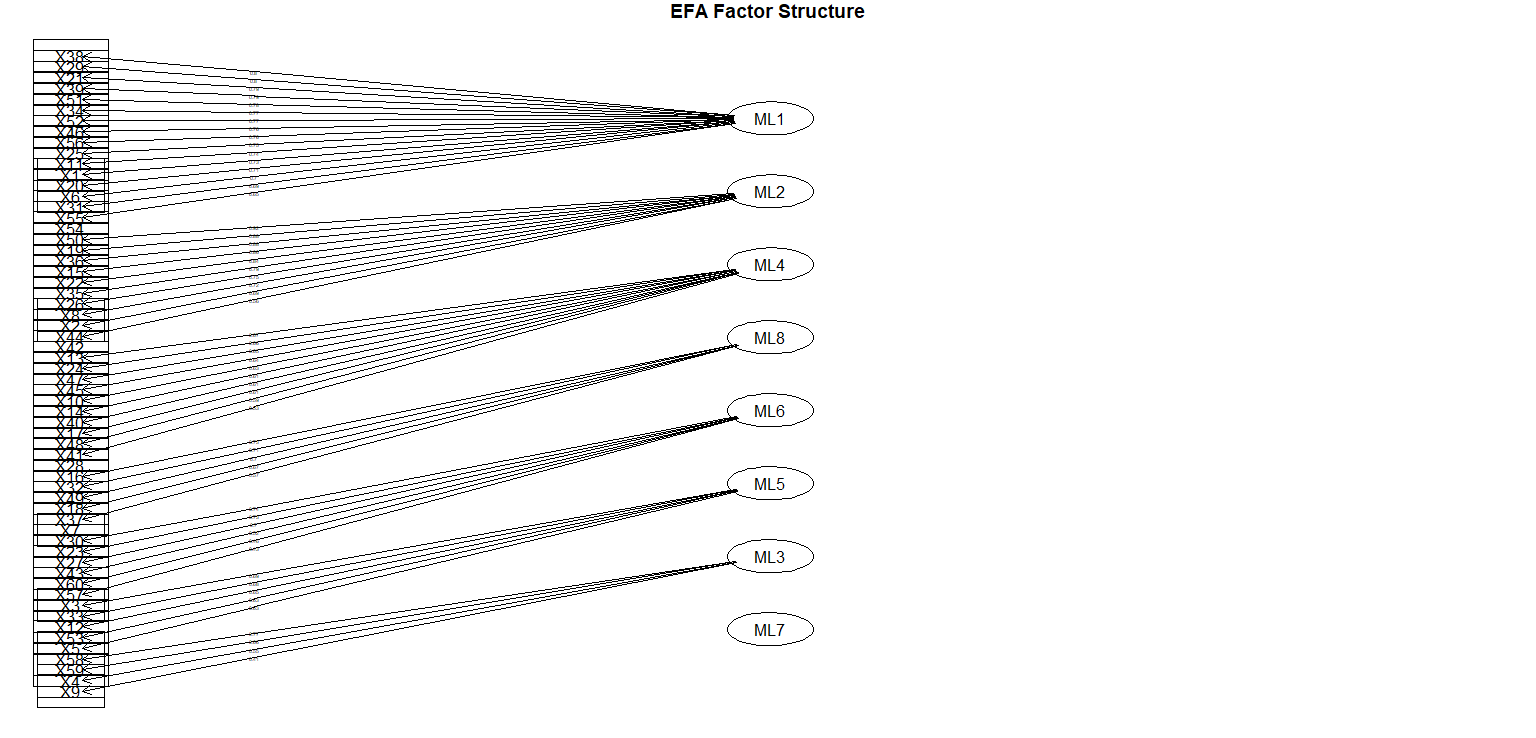
\includegraphics[width=1.5\linewidth]{../../assets/images/EFA_ML.png}
        \caption{Biểu đồ EFA tổng quát}
        \label{fig:efa_general}
\end{figure}

\subsection{Bước 6: Đánh giá độ tin cậy Cronbach's Alpha}

Đánh giá độ tin cậy cho từng nhân tố được trích xuất từ EFA:

\begin{figure}[h!]
    \centering
        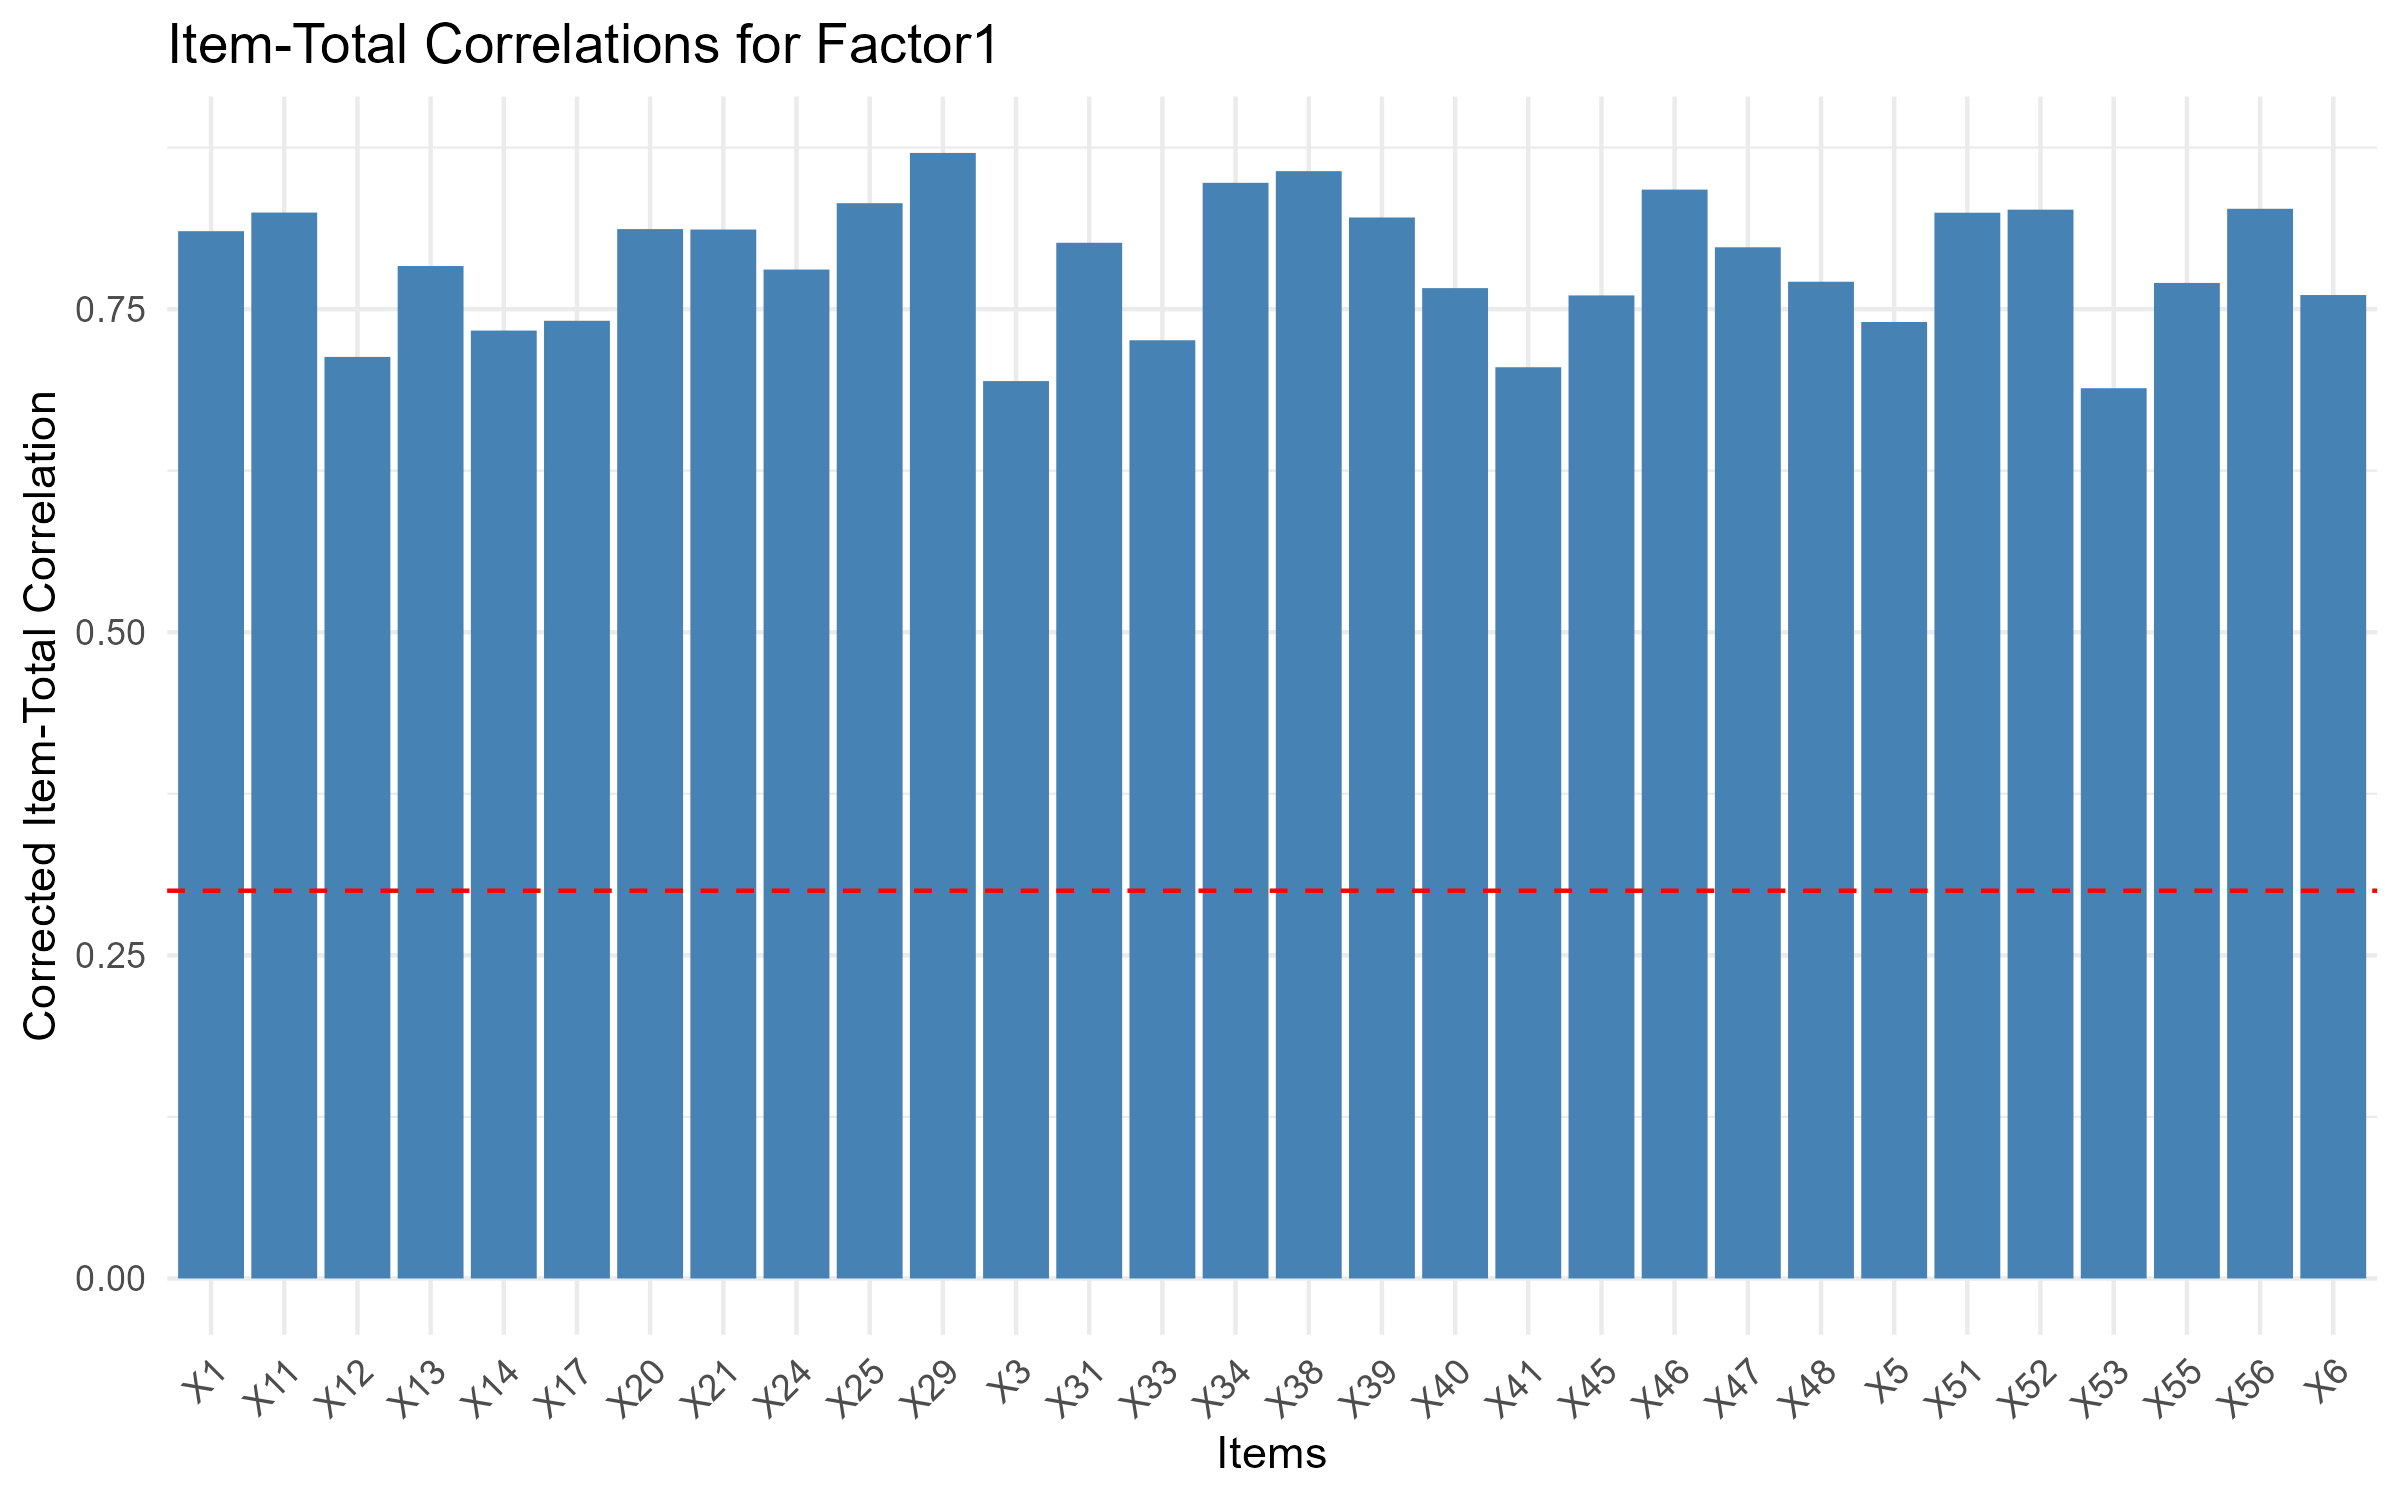
\includegraphics[width=0.55\linewidth]{../../assets/images/reliability_Factor1.png}
        \caption{Độ tin cậy Factor 1}
        \label{fig:reliability_f1}
\end{figure}

\begin{figure}[h!]
    \centering
    % Hàng 1 của 6 hình còn lại
    \begin{subfigure}[b]{0.45\linewidth}
        \centering
        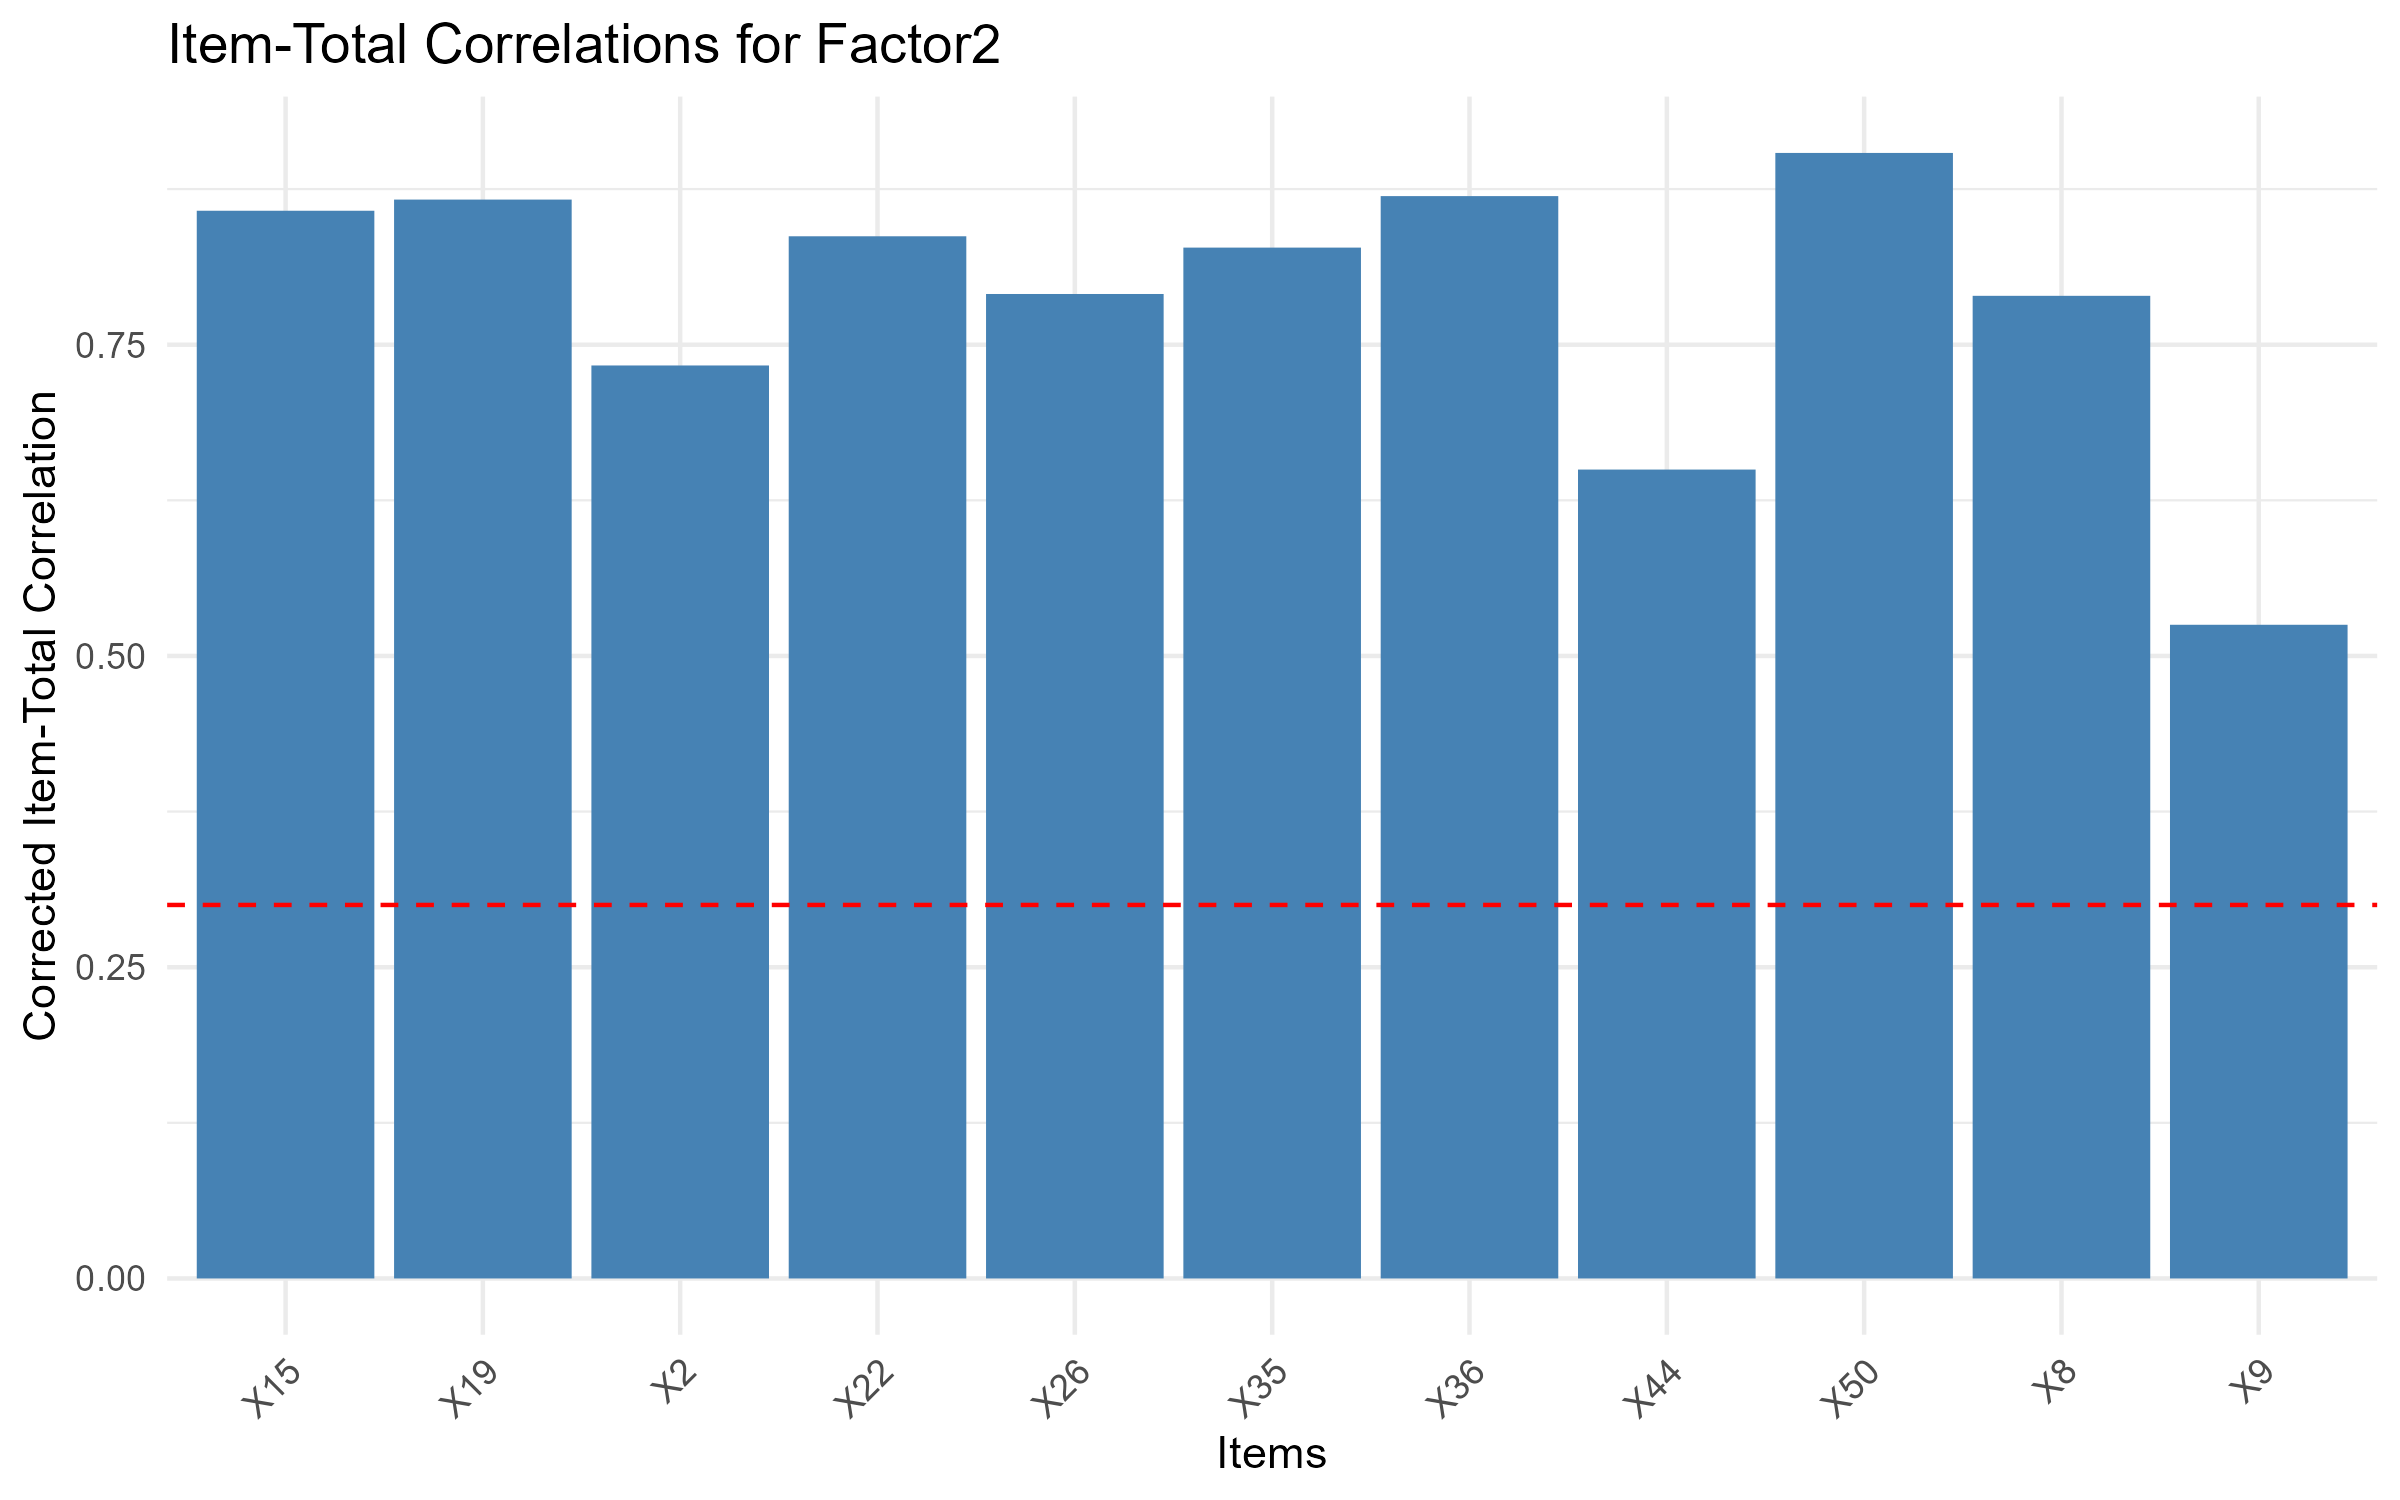
\includegraphics[width=\linewidth]{../../assets/images/reliability_Factor2.png}
        \caption{Độ tin cậy Factor 2}
        \label{fig:reliability_f2}
    \end{subfigure}
    \hfill
    \begin{subfigure}[b]{0.45\linewidth}
        \centering
        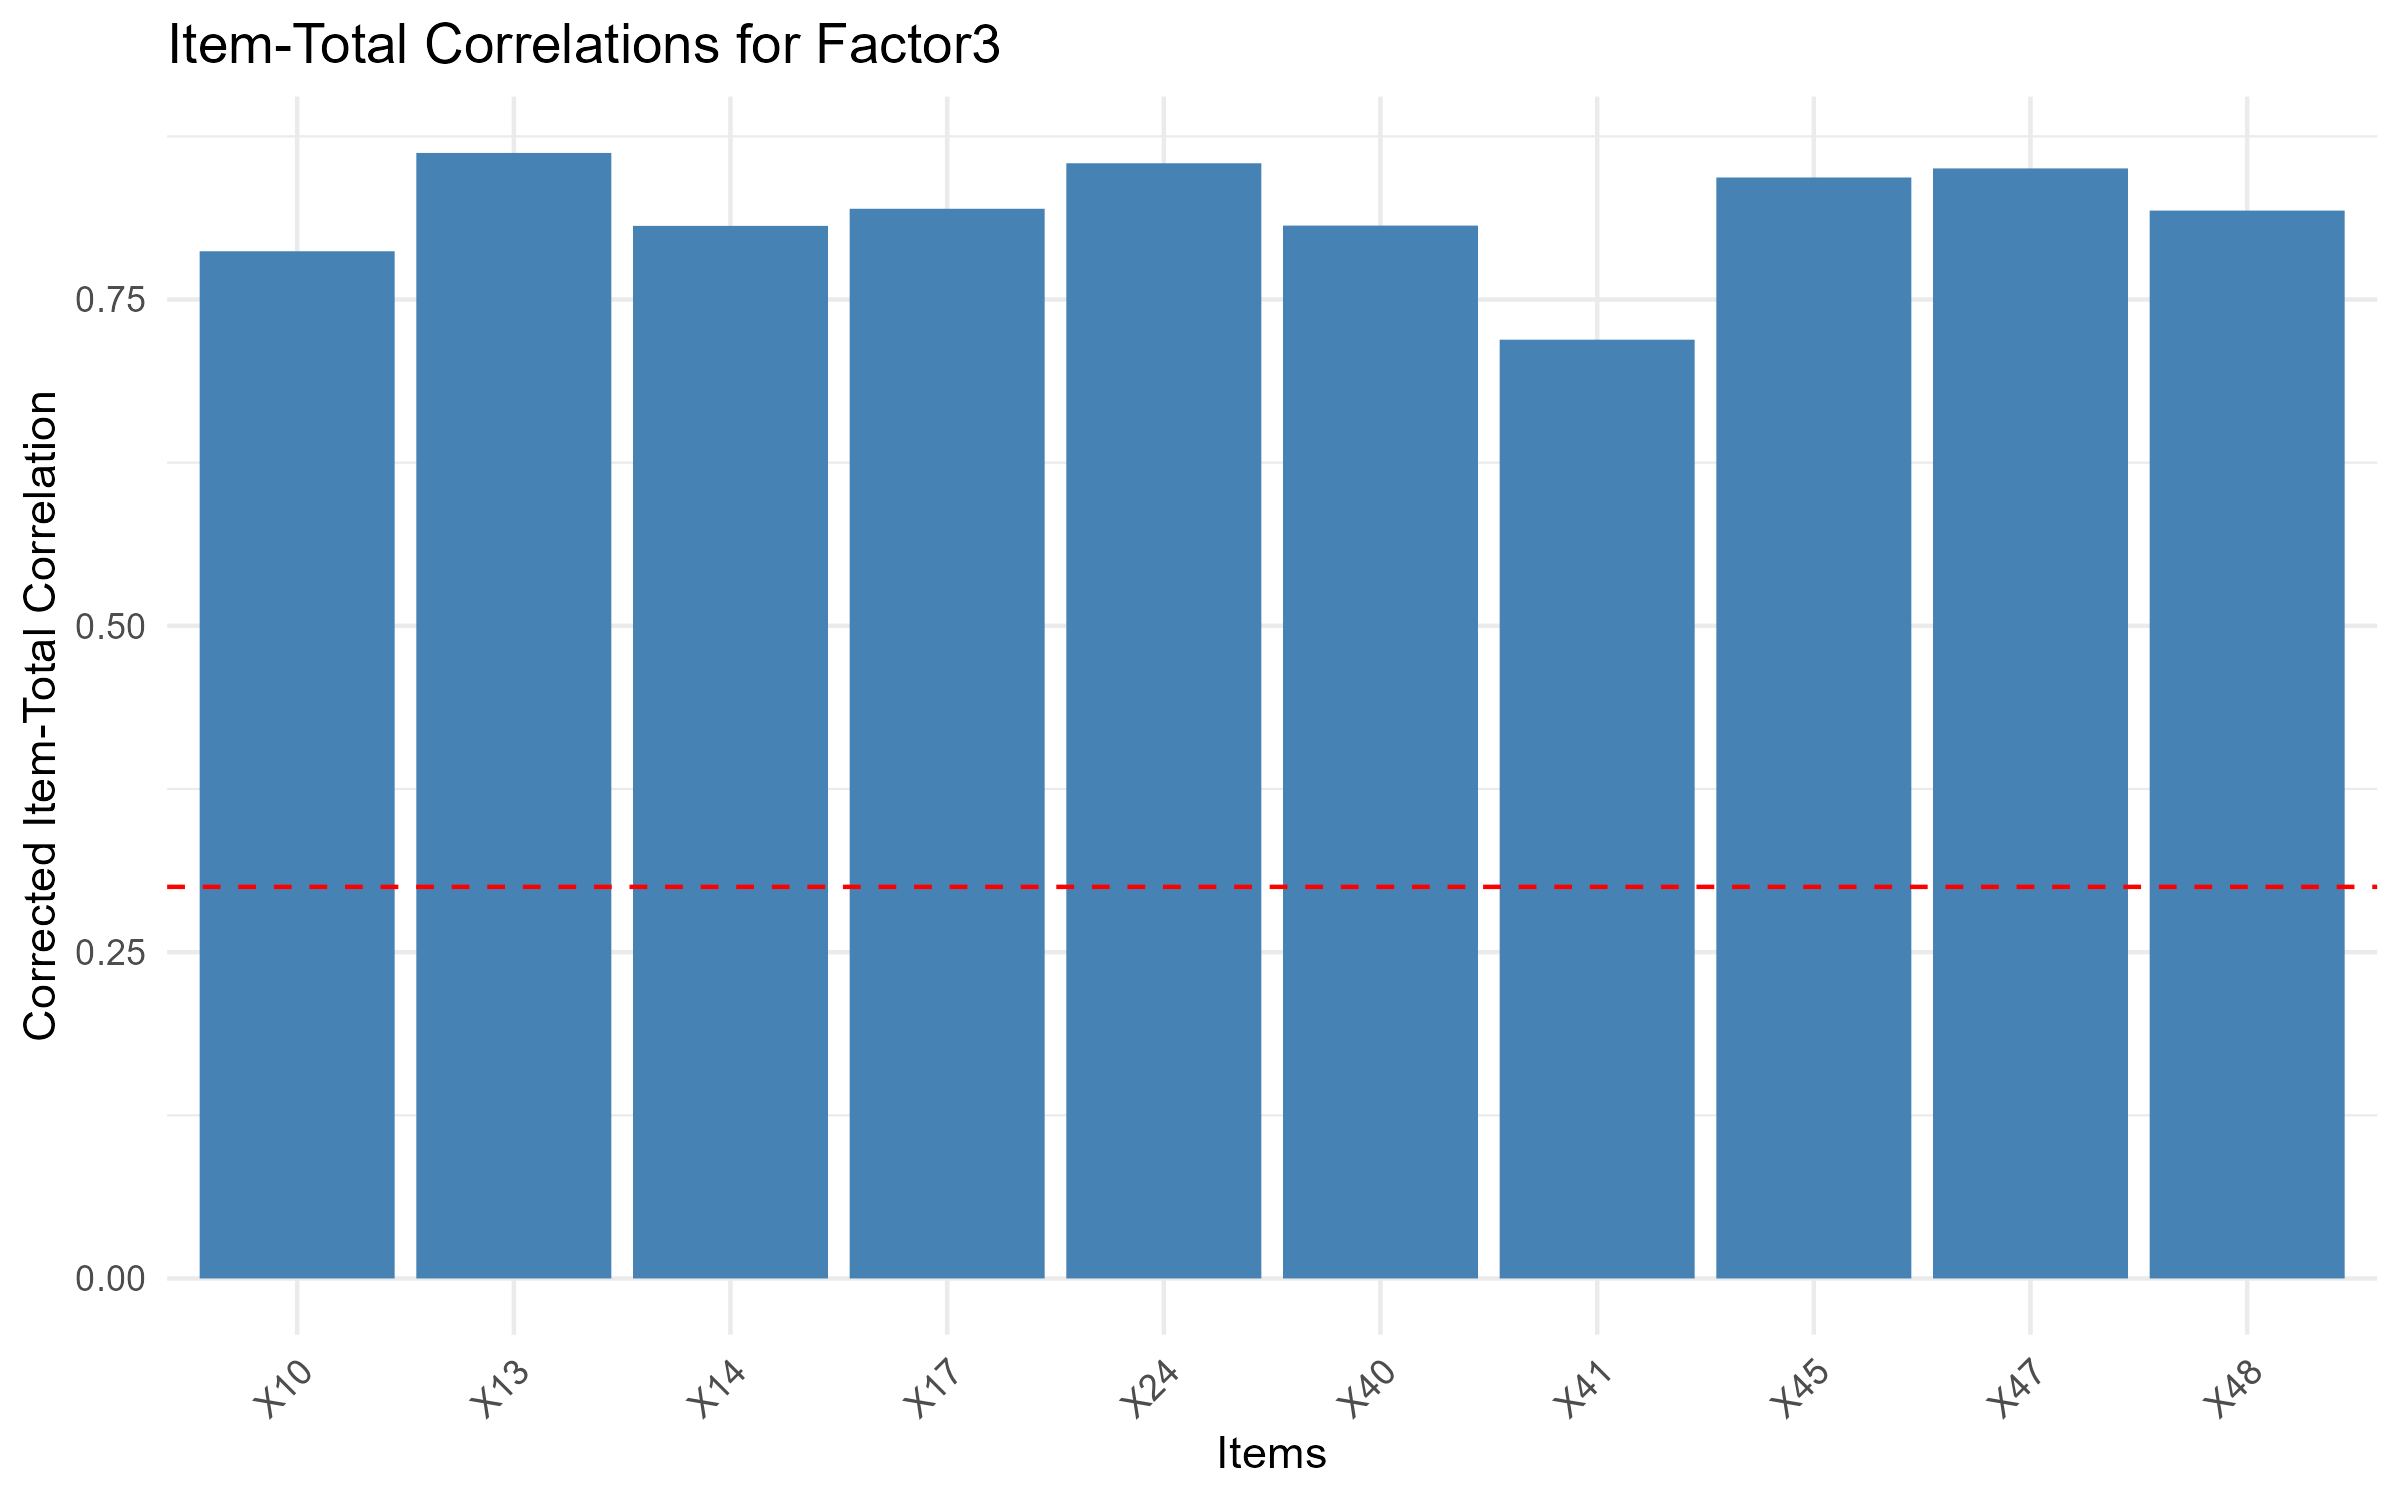
\includegraphics[width=\linewidth]{../../assets/images/reliability_Factor3.png}
        \caption{Độ tin cậy Factor 3}
        \label{fig:reliability_f3}
    \end{subfigure}

    \vskip 0.5cm
    % Hàng 2 của 6 hình còn lại
    \begin{subfigure}[b]{0.45\linewidth}
        \centering
        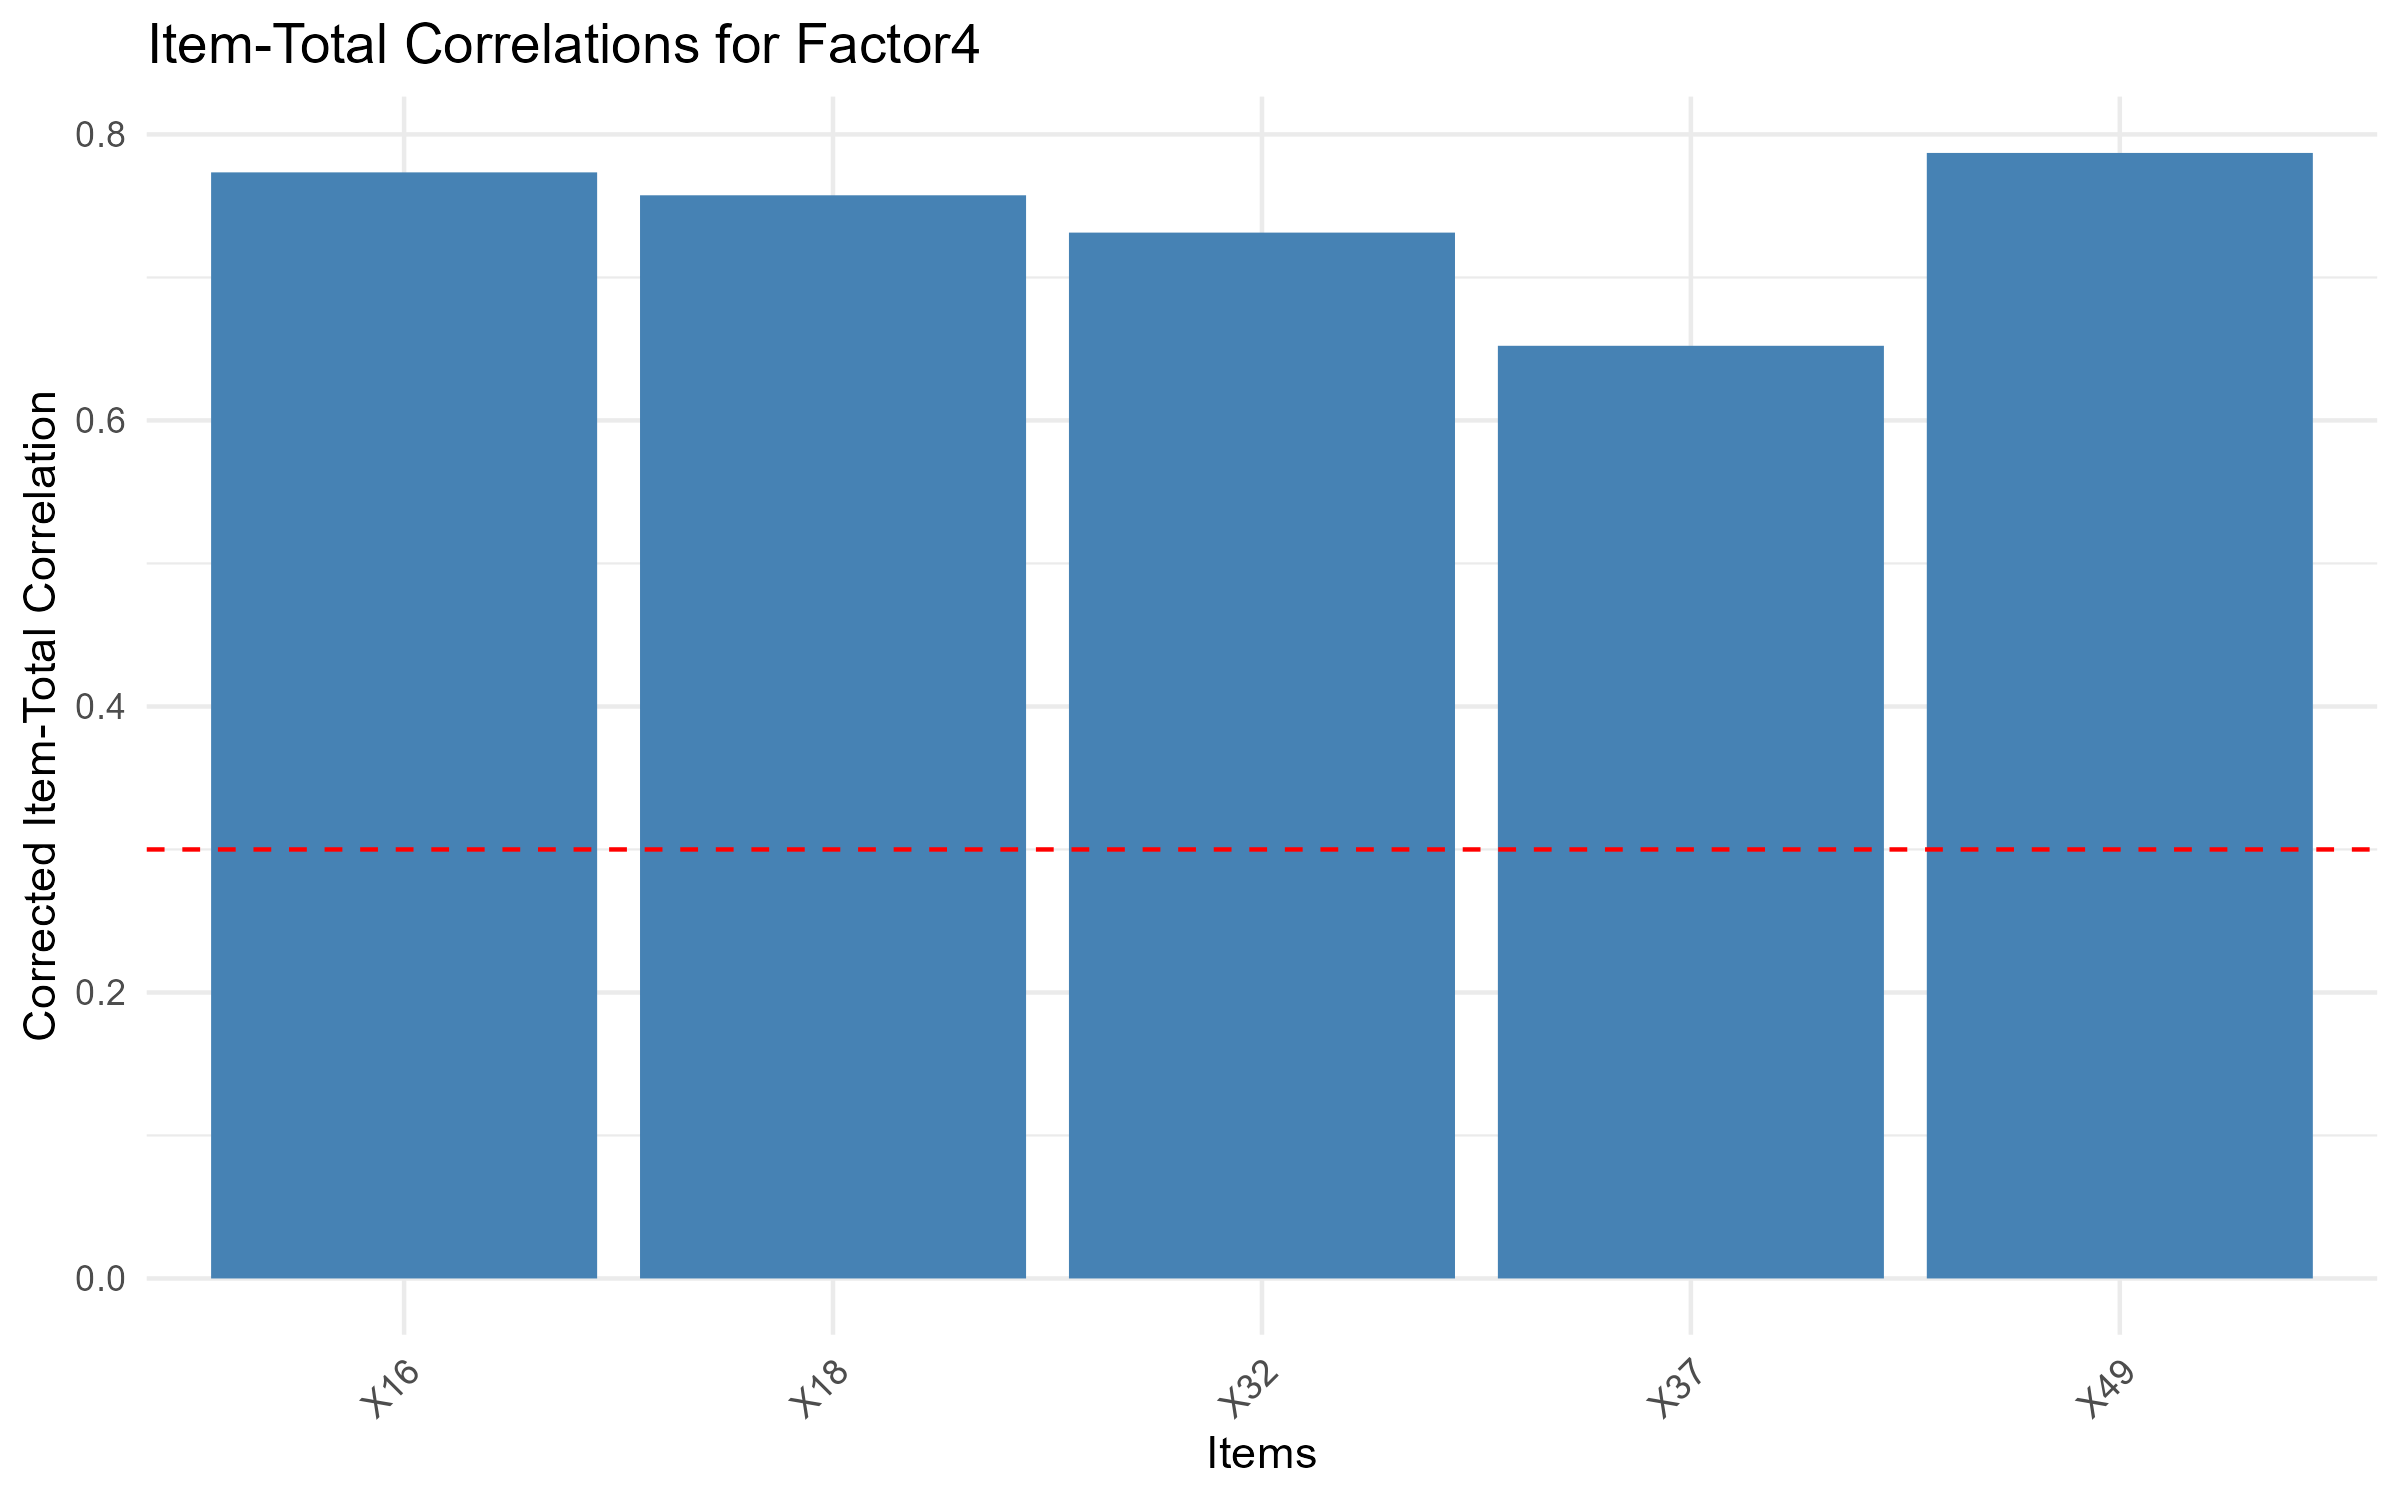
\includegraphics[width=\linewidth]{../../assets/images/reliability_Factor4.png}
        \caption{Độ tin cậy Factor 4}
        \label{fig:reliability_f4}
    \end{subfigure}
    \hfill
    \begin{subfigure}[b]{0.45\linewidth}
        \centering
        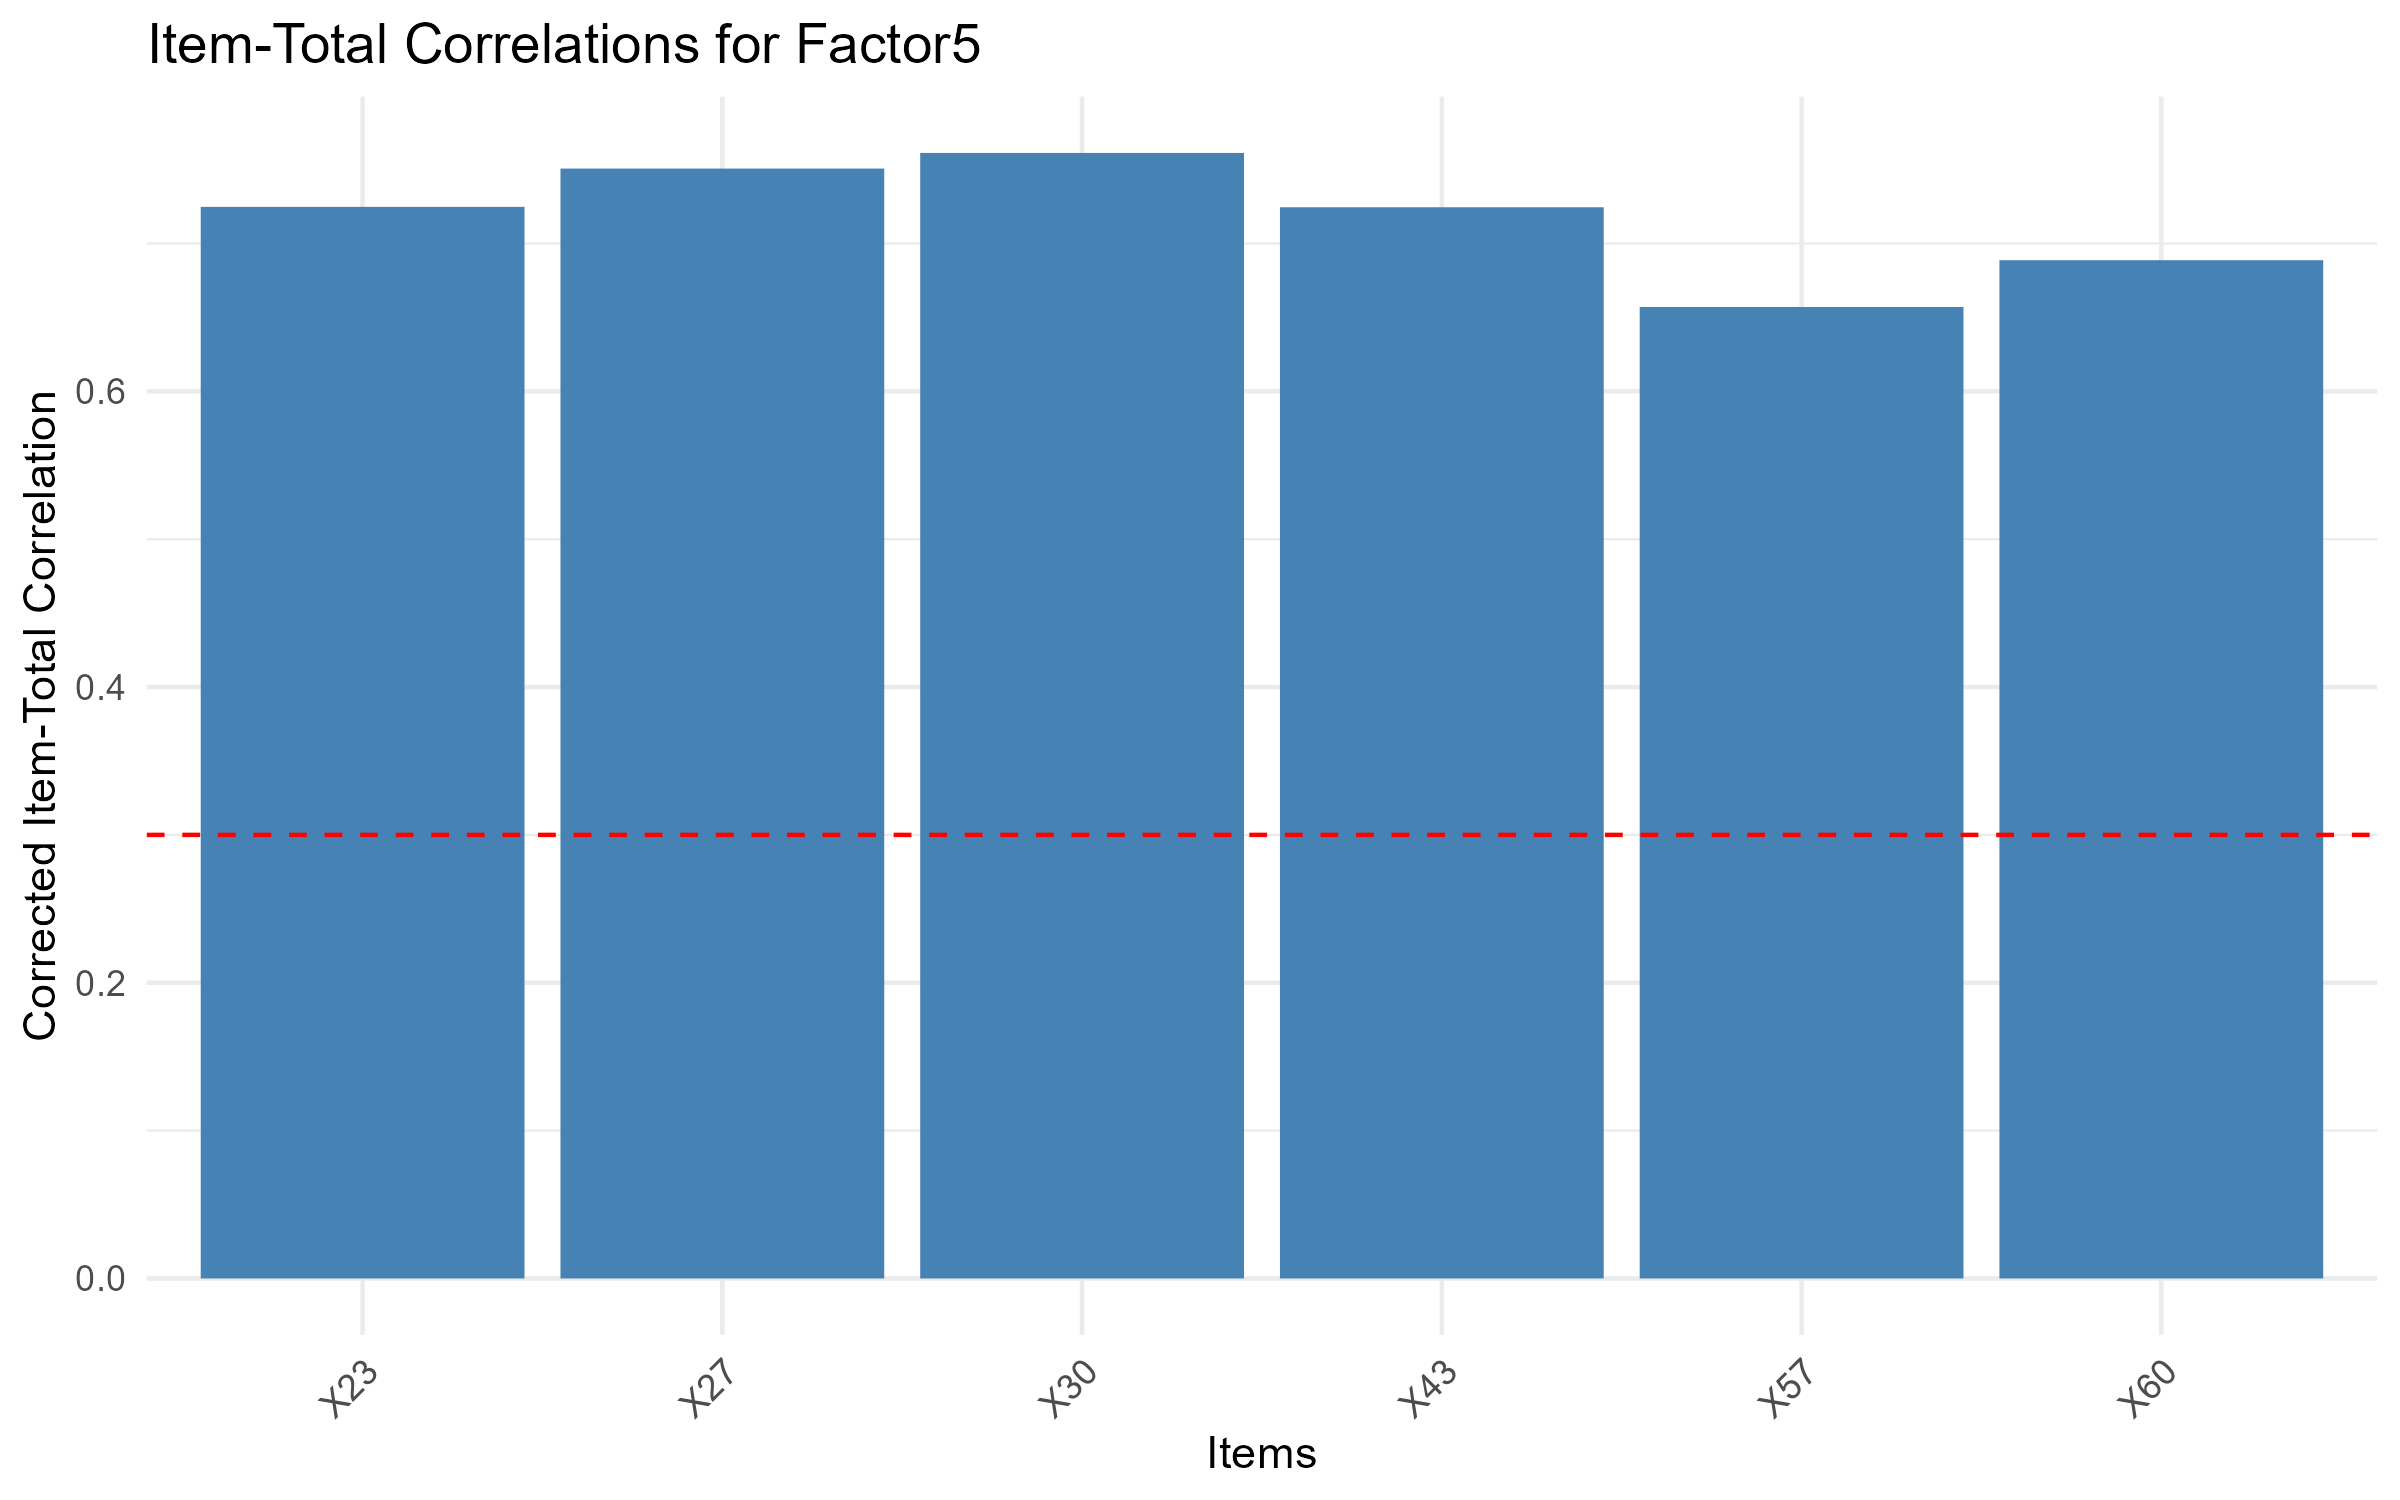
\includegraphics[width=\linewidth]{../../assets/images/reliability_Factor5.png}
        \caption{Độ tin cậy Factor 5}
        \label{fig:reliability_f5}
    \end{subfigure}

    \vskip 0.5cm
    % Hàng 3 của 6 hình còn lại
    \begin{subfigure}[b]{0.45\linewidth}
        \centering
        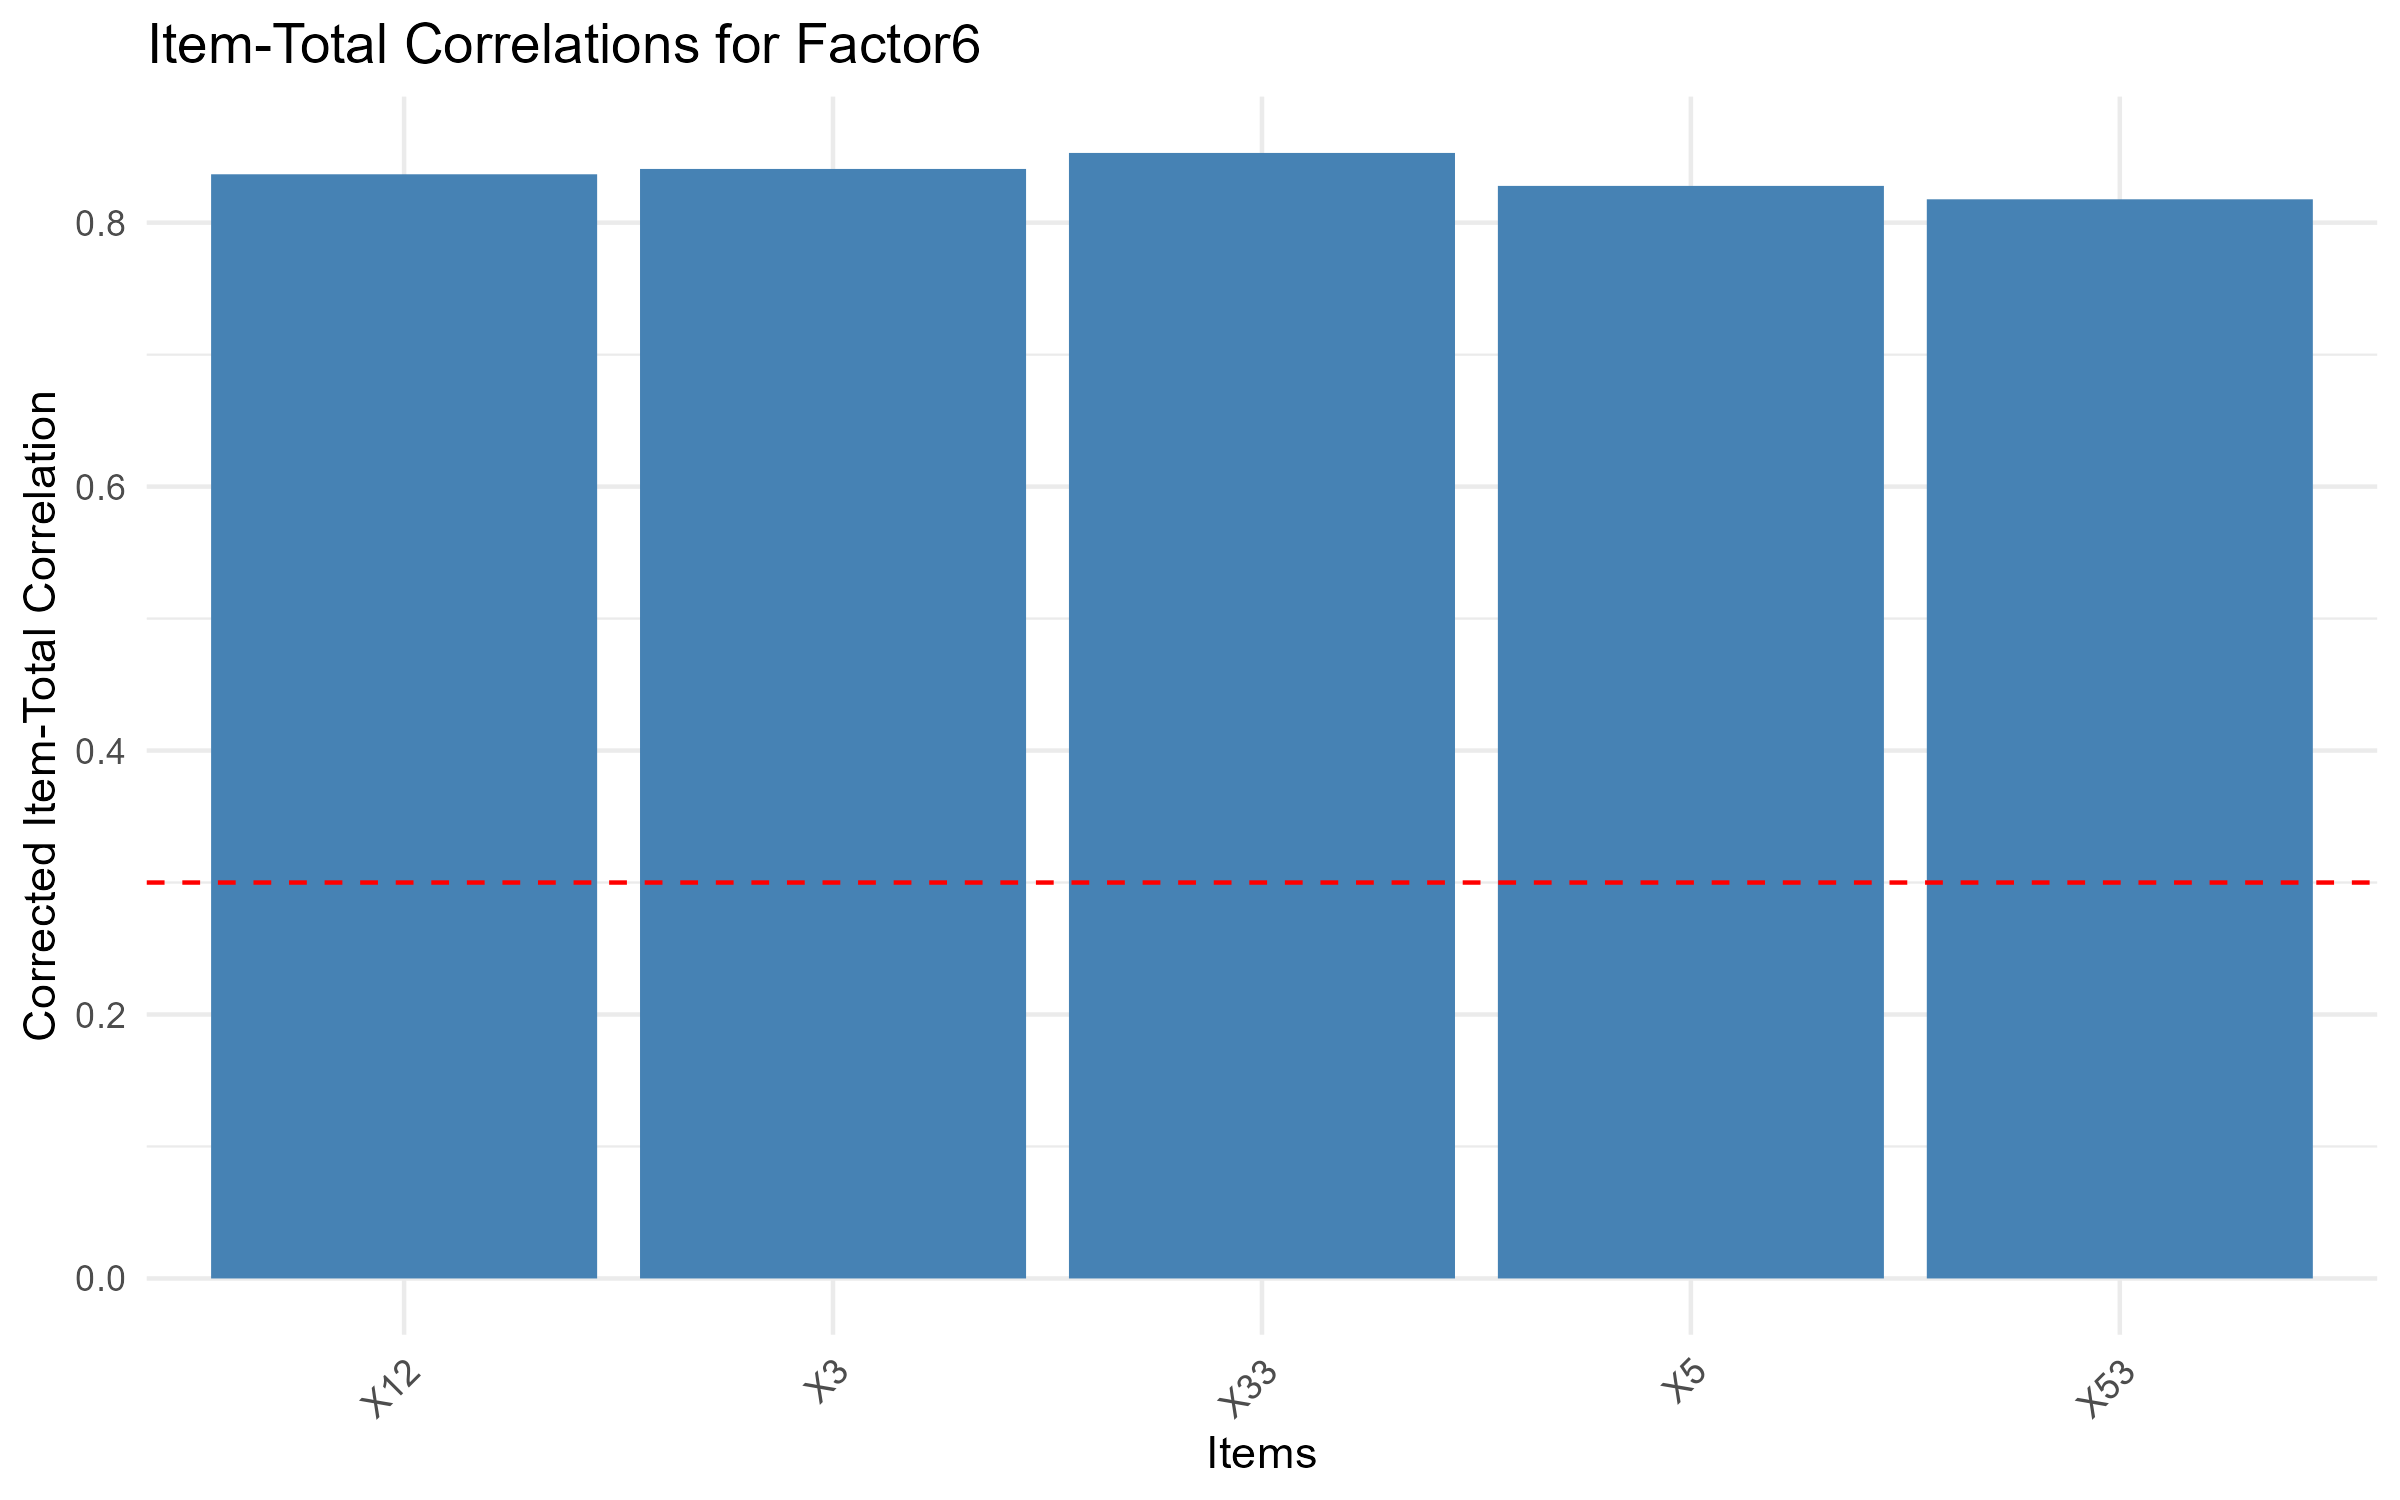
\includegraphics[width=\linewidth]{../../assets/images/reliability_Factor6.png}
        \caption{Độ tin cậy Factor 6}
        \label{fig:reliability_f6}
    \end{subfigure}
    \hfill
    \begin{subfigure}[b]{0.45\linewidth}
        \centering
        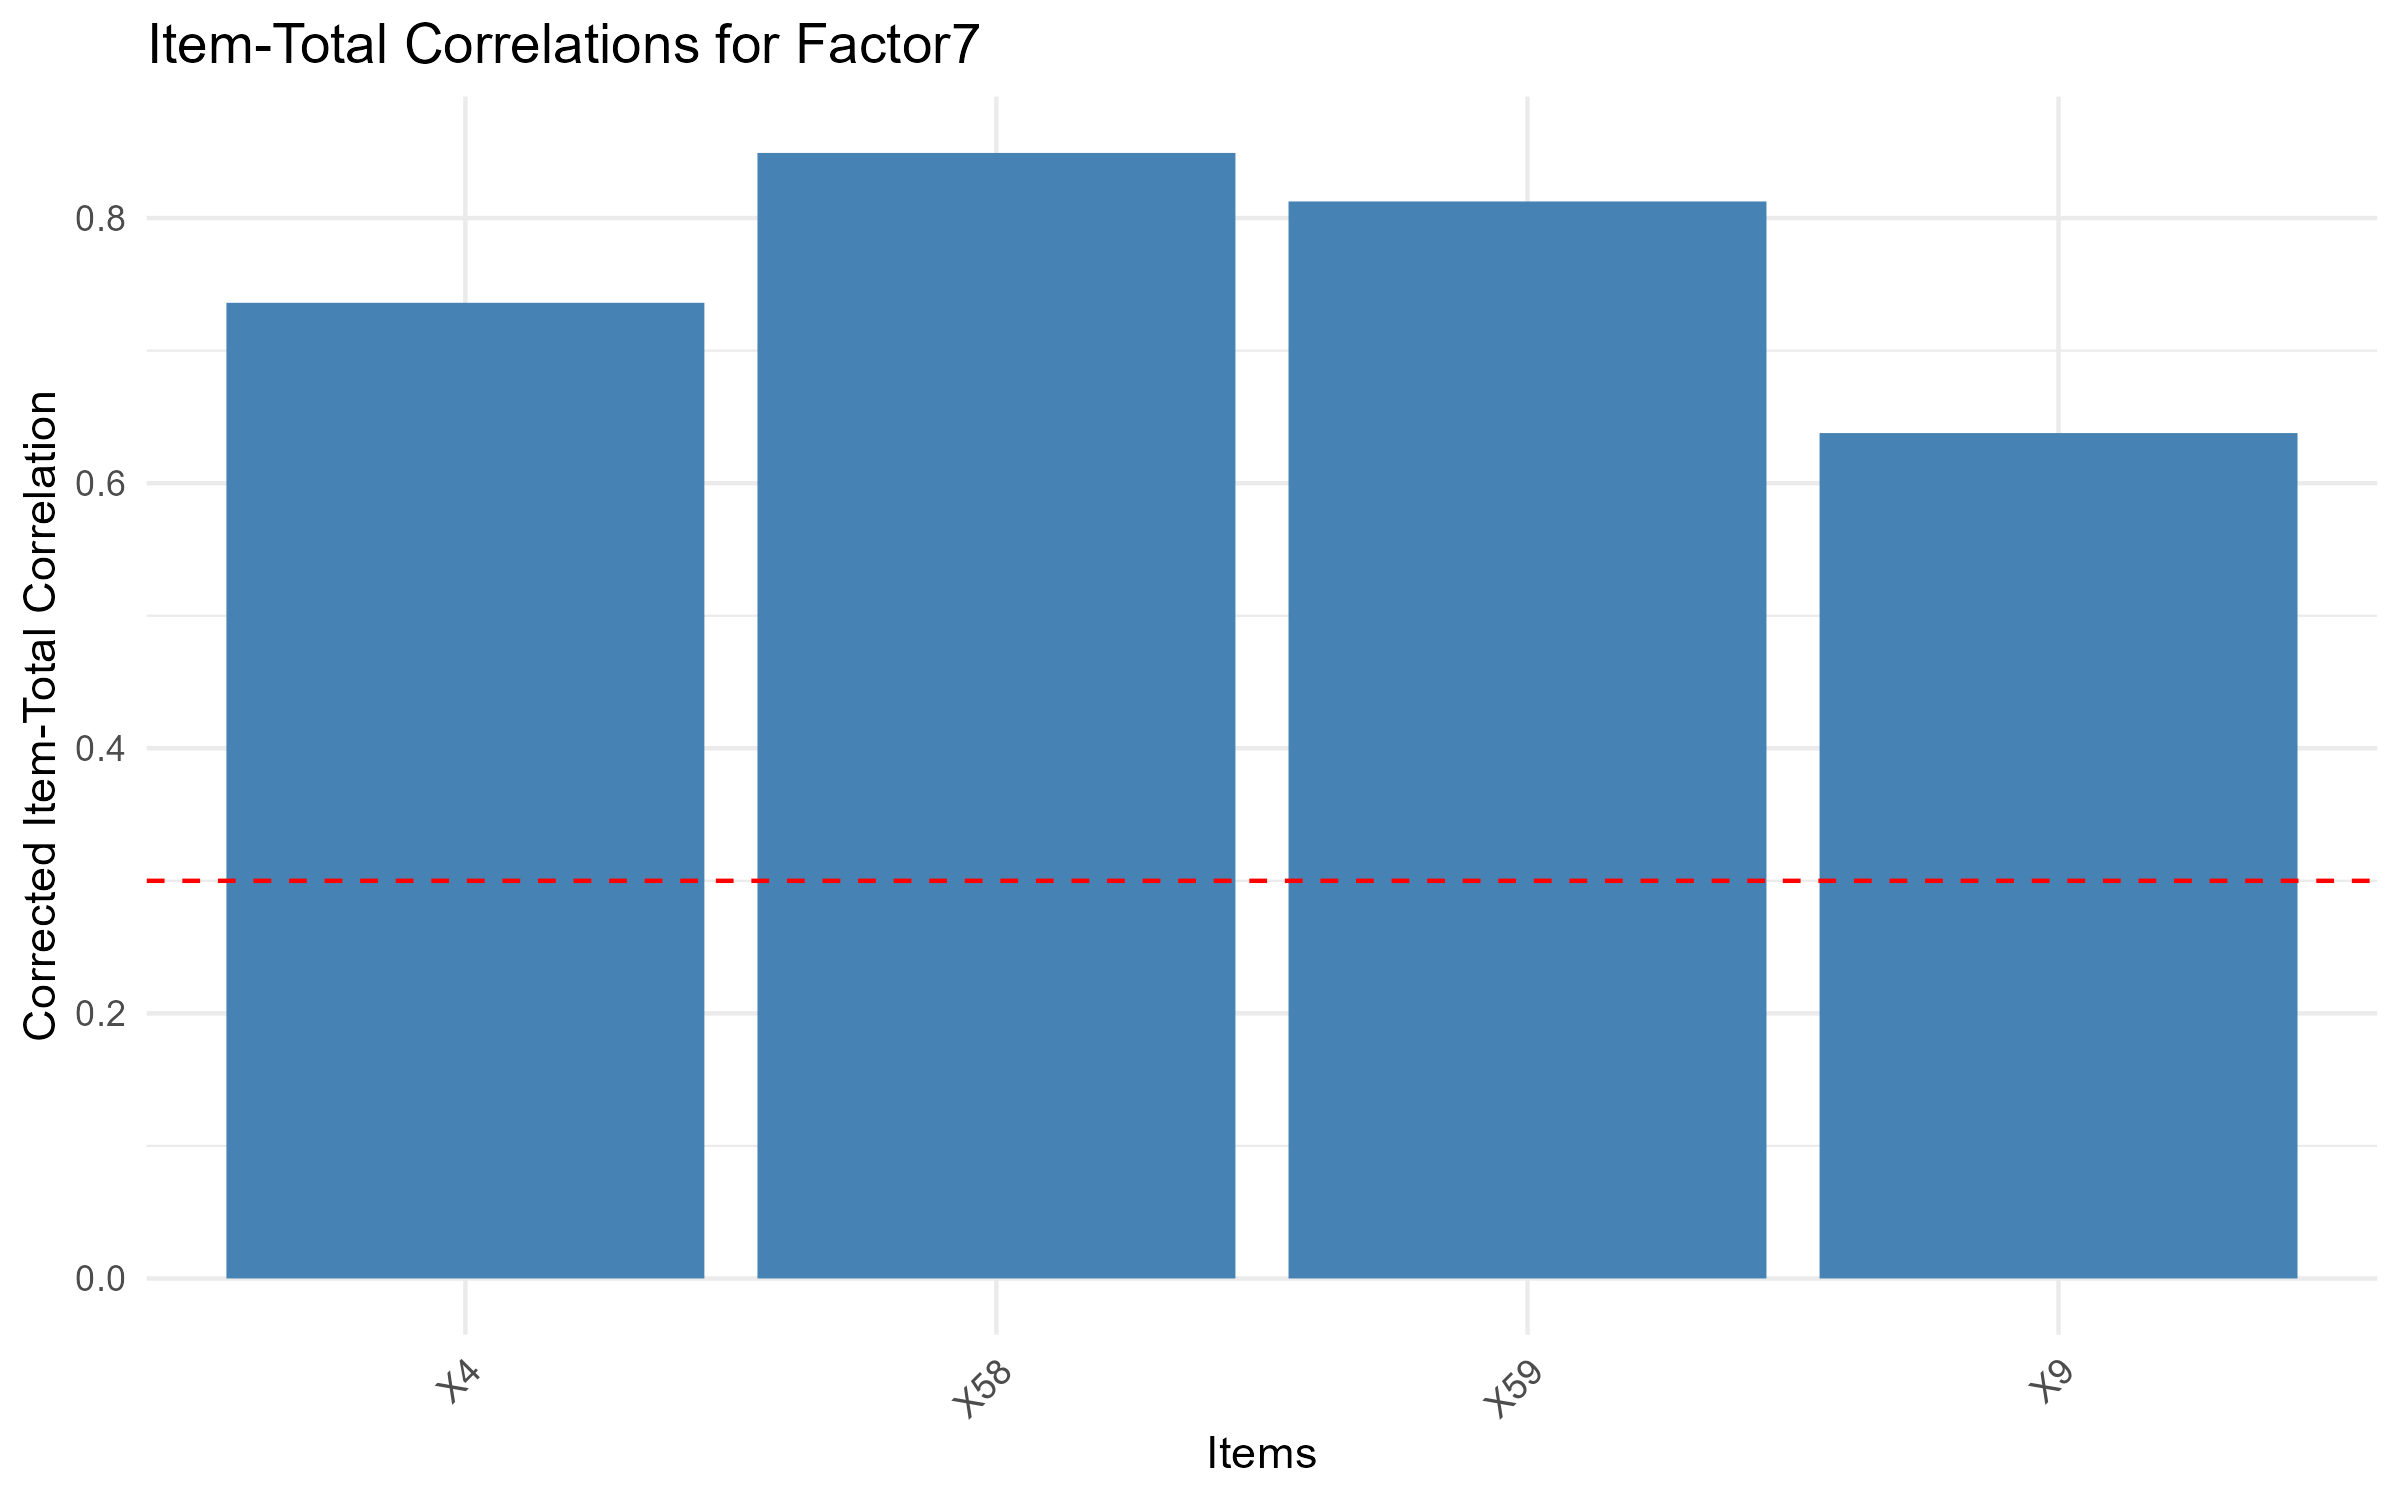
\includegraphics[width=\linewidth]{../../assets/images/reliability_Factor7.png}
        \caption{Độ tin cậy Factor 7}
        \label{fig:reliability_f7}
    \end{subfigure}

    \caption{Biểu đồ độ tin cậy từng nhân tố}
    \label{fig:efa_reliability}
\end{figure}

\subsection{Quy trình phân tích tổng hợp}

\subsection{Đánh giá hiệu quả mô hình}
\subsubsection*{Cross-validation cho PCA}
Đánh giá tính ổn định của các thành phần chính thông qua validation chéo.

\subsubsection*{Metrics cho clustering}
\begin{itemize}
    \item \textbf{Silhouette coefficient}: $s_i = \frac{b_i - a_i}{\max(a_i, b_i)}$
    \item \textbf{Calinski-Harabasz index}: $\frac{SS_B/(k-1)}{SS_W/(n-k)}$
    \item \textbf{Davies-Bouldin index}: $\frac{1}{k}\sum_{i=1}^k \max_{j \neq i} \frac{\sigma_i + \sigma_j}{d_{ij}}$
\end{itemize}

Quy trình phân tích dữ liệu nhiều chiều tổng hợp bao gồm nhiều bước từ khám phá dữ liệu ban đầu đến xây dựng mô hình cuối cùng. Mỗi kỹ thuật có ưu điểm riêng và cần được lựa chọn phù hợp với mục tiêu nghiên cứu cụ thể. Việc kết hợp nhiều phương pháp thường cho kết quả toàn diện và đáng tin cậy hơn.

\section{Phân tích nhân tố khám phá (EFA)}

EFA là một kỹ thuật thống kê được sử dụng để xác định cấu trúc ẩn trong một tập dữ liệu với nhiều biến quan sát \cite{vu2022, hair2019, tabachnick2019}.

\subsection{Mô hình phân tích nhân tố}

Mô hình EFA tương tự như mô hình factor analysis đã trình bày, nhưng tập trung vào việc khám phá số lượng và bản chất của các nhân tố mà không có giả định trước về cấu trúc.

\subsection{Kiểm định độ tin cậy Cronbach's Alpha}

Cronbach's Alpha là một thước đo độ tin cậy nội bộ của thang đo, đánh giá mức độ nhất quán giữa các mục trong cùng một nhân tố. Giá trị Alpha từ 0.7 trở lên được coi là chấp nhận được.

\section{Kết luận chương}

Chương này đã trình bày một cách hệ thống các phương pháp phân tích dữ liệu nhiều chiều quan trọng. Những điểm chính cần ghi nhớ:

\begin{itemize}
    \item \textbf{PCA} phù hợp cho giảm chiều và trực quan hóa dữ liệu
    \item \textbf{Factor Analysis} tập trung vào tìm cấu trúc tiềm ẩn trong dữ liệu quan sát
    \item \textbf{EFA} giúp khám phá số lượng và bản chất của các nhân tố ẩn
    \item Đánh giá độ tin cậy bằng Cronbach's Alpha để đảm bảo tính nhất quán nội bộ
    \item Việc kết hợp nhiều phương pháp thường cho hiểu biết sâu sắc hơn về dữ liệu
    \item Cần validation kỹ lưỡng để đảm bảo tính tin cậy của kết quả
\end{itemize}

Các kỹ thuật này tạo thành nền tảng vững chắc cho việc phân tích dữ liệu phức tạp, từ nghiên cứu khoa học đến các ứng dụng thực tiễn trong nhiều lĩnh vực khác nhau.

% Kết luận
\chapter*{KẾT LUẬN}
\addcontentsline{toc}{chapter}{KẾT LUẬN}

Thống kê nâng cao đóng vai trò then chốt trong việc phân tích và giải thích dữ liệu phức tạp trong thời đại khoa học dữ liệu hiện đại. Qua quá trình nghiên cứu và tìm hiểu các phương pháp thống kê tiên tiến, bài thu hoạch này đã cung cấp một cái nhìn toàn diện về lý thuyết và ứng dụng thực tiễn của thống kê nâng cao.

\section*{Tổng kết kiến thức đã trình bày}

Bài thu hoạch đã trình bày một cách có hệ thống ba nhóm kiến thức cốt lõi của thống kê nâng cao:

\subsection*{Kiến thức nền tảng vững chắc}

Chương 1 đã củng cố và mở rộng các khái niệm cơ bản về lý thuyết xác suất và thống kê toán học. Những nội dung chính bao gồm:

\begin{itemize}
    \item \textbf{Không gian xác suất và biến ngẫu nhiên}: Xây dựng nền tảng toán học vững chắc cho việc mô hình hóa các hiện tượng ngẫu nhiên, từ định nghĩa không gian xác suất $(\Omega, \mathcal{F}, P)$ đến các tính chất quan trọng của biến ngẫu nhiên.
    
    \item \textbf{Phân phối xác suất quan trọng}: Tìm hiểu sâu về các phân phối thường gặp như phân phối chuẩn, chi-bình phương, Student, và F, cùng với các tính chất đặc trưng và ứng dụng của chúng trong kiểm định thống kê.
    
    \item \textbf{Định lý giới hạn trung tâm và luật số lớn}: Hiểu rõ hai định lý cơ bản nhất của lý thuyết xác suất, giải thích tại sao phân phối chuẩn có vai trò quan trọng trong thống kê ứng dụng và cách chúng tạo nền tảng cho các phương pháp suy diễn thống kê.
    
    \item \textbf{Cơ sở kiểm định giả thuyết}: Nắm vững quy trình kiểm định từ việc thiết lập giả thuyết đến ra quyết định, hiểu rõ về các loại sai lầm và ý nghĩa của p-value.
\end{itemize}

\subsection*{Phương pháp kiểm định thống kê}

Chương 2 đã trình bày chi tiết các phương pháp kiểm định quan trọng với cả lý thuyết và ứng dụng thực tiễn:

\begin{itemize}
    \item \textbf{Kiểm định Pearson chi-bình phương}: Nắm vững cách áp dụng cho kiểm định tính phù hợp phân phối (goodness-of-fit) và kiểm định độc lập trong bảng chéo, với các điều kiện áp dụng và cách giải thích kết quả.
    
    \item \textbf{Kiểm định Kolmogorov-Smirnov}: Hiểu rõ ưu điểm của phương pháp phi tham số này trong việc so sánh phân phối liên tục, đặc biệt khi không có giả định về dạng phân phối cụ thể.
    
    \item \textbf{Ứng dụng thực tế với dữ liệu phức tạp}: Thông qua việc phân tích các bộ dữ liệu Singletons, Binaires và Meteo, đã thấy được cách áp dụng các phương pháp kiểm định trong các mô hình phức tạp với nhiều biến phụ thuộc.
    
    \item \textbf{Mô phỏng Monte Carlo}: Sử dụng MATLAB để minh họa và kiểm chứng các kết quả lý thuyết, đồng thời đánh giá hiệu quả của các phương pháp kiểm định trong các tình huống khác nhau.
\end{itemize}

\subsection*{Phân tích dữ liệu nhiều chiều}

Chương 3 đã giới thiệu các kỹ thuật tiên tiến trong phân tích dữ liệu nhiều chiều:

\begin{itemize}
    \item \textbf{Phân tích thành phần chính (PCA)}: Nắm vững phương pháp giảm chiều dữ liệu hiệu quả, từ cơ sở toán học đến các tiêu chí lựa chọn số thành phần và ứng dụng trong trực quan hóa dữ liệu.
    
    \item \textbf{Phân tích nhân tố (Factor Analysis)}: Hiểu rõ sự khác biệt giữa FA và PCA, cách xây dựng mô hình nhân tố và các phương pháp xoay nhân tố để có được kết quả dễ giải thích hơn.
    
    \item \textbf{Phân tích nhân tố khám phá (EFA)}: Áp dụng thành công trên dữ liệu thực tế về đánh giá dịch vụ thư viện, từ việc kiểm định các giả định ban đầu đến trích xuất các nhân tố có ý nghĩa và đánh giá độ tin cậy.
    
    \item \textbf{Công cụ tính toán}: Sử dụng thành thạo R trong việc thực hiện các phân tích phức tạp, từ kiểm định KMO và Bartlett đến visualization các kết quả phân tích.
\end{itemize}

\section*{Ý nghĩa và ứng dụng của thống kê nâng cao}

\subsection*{Đóng góp vào nghiên cứu khoa học}

Thống kê nâng cao cung cấp những công cụ mạnh mẽ cho nghiên cứu khoa học hiện đại:

\begin{itemize}
    \item \textbf{Xử lý dữ liệu lớn và phức tạp}: Các phương pháp như PCA và EFA cho phép nghiên cứu viên làm việc với datasets có hàng trăm biến số, trích xuất thông tin có ý nghĩa từ dữ liệu nhiều chiều.
    
    \item \textbf{Kiểm chứng giả thuyết nghiên cứu}: Các phương pháp kiểm định tiên tiến giúp đánh giá độ tin cậy của các phát hiện nghiên cứu, kiểm soát tỷ lệ sai lầm trong nghiên cứu đa so sánh.
    
    \item \textbf{Mô hình hóa mối quan hệ phức tạp}: Thống kê nâng cao cho phép mô tả và phân tích các mối quan hệ phi tuyến, tương tác giữa nhiều biến số đồng thời.
\end{itemize}

\subsection*{Ứng dụng trong thực tiễn}

Các phương pháp đã học có ứng dụng rộng rãi trong nhiều lĩnh vực:

\begin{itemize}
    \item \textbf{Kinh doanh và marketing}: Phân tích hành vi khách hàng, phân khúc thị trường, đánh giá hiệu quả chương trình marketing thông qua các kỹ thuật clustering và factor analysis.
    
    \item \textbf{Y học và sức khỏe cộng đồng}: Phân tích dữ liệu lâm sàng, nghiên cứu dịch tễ học, đánh giá hiệu quả điều trị thông qua các phương pháp kiểm định tiên tiến.
    
    \item \textbf{Khoa học xã hội}: Nghiên cứu tâm lý, giáo dục, xã hội học sử dụng EFA để xây dựng và validation các thang đo, đánh giá chất lượng dịch vụ công.
    
    \item \textbf{Kỹ thuật và công nghệ}: Kiểm soát chất lượng, tối ưu hóa quy trình, phân tích độ tin cậy hệ thống thông qua các phương pháp thống kê tiên tiến.
\end{itemize}

\section*{Hạn chế và thử thách}

Mặc dù có nhiều ưu điểm, thống kê nâng cao cũng đối mặt với một số hạn chế:

\subsection*{Về mặt lý thuyết}

\begin{itemize}
    \item \textbf{Giả định nghiêm ngặt}: Nhiều phương pháp yêu cầu các giả định về phân phối dữ liệu, tính độc lập, và đồng phương sai có thể không được thỏa mãn trong thực tế.
    
    \item \textbf{Độ phức tạp tính toán}: Các thuật toán tối ưu hóa trong ML estimation, xoay nhân tố có thể gặp vấn đề hội tụ hoặc local optima.
    
    \item \textbf{Vấn đề đa so sánh}: Khi thực hiện nhiều kiểm định đồng thời, cần có các phương pháp điều chỉnh phù hợp để kiểm soát tỷ lệ sai lầm.
\end{itemize}

\subsection*{Về mặt ứng dụng}

\begin{itemize}
    \item \textbf{Giải thích kết quả}: Việc diễn giải ý nghĩa của các thành phần chính hoặc nhân tố đòi hỏi kiến thức chuyên môn sâu về lĩnh vực nghiên cứu.
    
    \item \textbf{Lựa chọn phương pháp}: Sự đa dạng của các phương pháp có thể gây khó khăn trong việc lựa chọn kỹ thuật phù hợp nhất cho từng bài toán cụ thể.
    
    \item \textbf{Chất lượng dữ liệu}: Kết quả phân tích phụ thuộc rất nhiều vào chất lượng dữ liệu đầu vào, đòi hỏi quy trình tiền xử lý cẩn thận.
\end{itemize}

\section*{Hướng phát triển trong tương lai}

\subsection*{Xu hướng công nghệ}

\begin{itemize}
    \item \textbf{Tích hợp với Machine Learning}: Kết hợp các phương pháp thống kê truyền thống với các thuật toán học máy để xử lý dữ liệu lớn và phức tạp hơn.
    
    \item \textbf{Thống kê Bayesian}: Phát triển các phương pháp suy diễn Bayesian cho phép cập nhật kiến thức một cách linh hoạt khi có thêm dữ liệu mới.
    
    \item \textbf{Phân tích dữ liệu thời gian thực}: Phát triển các thuật toán có thể xử lý và phân tích dữ liệu streaming với tốc độ cao.
\end{itemize}

\subsection*{Ứng dụng mới}

\begin{itemize}
    \item \textbf{Big Data Analytics}: Mở rộng các phương pháp truyền thống để làm việc với datasets có kích thước terabyte hoặc petabyte.
    
    \item \textbf{Artificial Intelligence}: Sử dụng thống kê nâng cao trong việc phát triển và đánh giá các mô hình AI, đặc biệt trong việc hiểu và giải thích tính năng của black-box models.
    
    \item \textbf{Interdisciplinary Research}: Áp dụng vào các lĩnh vực mới như bioinformatics, computational neuroscience, digital humanities.
\end{itemize}

\section*{Kết luận tổng quát}

Qua quá trình nghiên cứu chuyên đề "Thống kê nâng cao", em đã có được những hiểu biết sâu sắc về lý thuyết và ứng dụng của các phương pháp thống kê tiên tiến. Bài thu hoạch này không chỉ cung cấp kiến thức lý thuyết vững chắc mà còn thể hiện khả năng áp dụng thực tiễn thông qua việc sử dụng các công cụ tính toán như MATLAB và R.

\subsection*{Những thành tựu đạt được}

\begin{itemize}
    \item \textbf{Nắm vững lý thuyết}: Hiểu rõ các khái niệm cơ bản và nâng cao của thống kê toán học, từ lý thuyết xác suất đến các phương pháp phân tích nhiều chiều.
    
    \item \textbf{Kỹ năng ứng dụng}: Thành thạo trong việc sử dụng các công cụ tính toán để giải quyết các bài toán thống kê phức tạp.
    
    \item \textbf{Tư duy phản biện}: Phát triển khả năng đánh giá độ tin cậy của phương pháp, nhận biết hạn chế và lựa chọn kỹ thuật phù hợp.
    
    \item \textbf{Liên kết lý thuyết-thực tiễn}: Hiểu được cách áp dụng các phương pháp lý thuyết vào giải quyết các vấn đề thực tế.
\end{itemize}

\subsection*{Ý nghĩa đối với sự phát triển cá nhân}

Việc học tập chuyên đề này đã:

\begin{itemize}
    \item Nâng cao khả năng tư duy logic và phân tích định lượng
    \item Chuẩn bị nền tảng vững chắc cho các nghiên cứu khoa học trong tương lai
    \item Phát triển kỹ năng sử dụng công cụ tính toán chuyên nghiệp
    \item Tạo điều kiện cho việc ứng dụng thống kê trong nhiều lĩnh vực khác nhau
\end{itemize}

\subsection*{Cam kết phát triển tiếp}

Với nền tảng kiến thức đã xây dựng, em cam kết:

\begin{itemize}
    \item Tiếp tục nghiên cứu sâu hơn về các phương pháp thống kê tiên tiến
    \item Ứng dụng các kiến thức đã học vào các dự án nghiên cứu cụ thể
    \item Cập nhật những phát triển mới nhất trong lĩnh vực khoa học dữ liệu
    \item Chia sẻ kiến thức và kinh nghiệm với cộng đồng nghiên cứu
\end{itemize}

Thống kê nâng cao không chỉ là một môn học, mà là một công cụ mạnh mẽ giúp chúng ta hiểu và giải thích thế giới xung quanh thông qua dữ liệu. Trong thời đại mà dữ liệu trở thành tài sản quý giá nhất, việc nắm vững các phương pháp thống kê nâng cao là điều kiện cần thiết cho bất kỳ ai muốn đóng góp vào sự phát triển của khoa học và xã hội.

% Tài liệu tham khảo
*Trích dẫn lần sau:
(FAO, 1977)
 & United States Government Accountability Office (2019)

*Trích dẫn lần đầu:
Food and Agriculture Organization of the United Nations (FAO, 2020)

*Trích dẫn lần sau:
FAO (1977)
 \\
      \hline
       \textbf{Nhiều tài liệu}
       
Sắp xếp các tài liệu theo năm xuất bản tăng dần. Nếu các tài liệu có cùng năm xuất bản, thì sắp xếp theo thứ tự bảng chữ cái.
  & (Hồng và ctv. 2014; Hiền và ctv., 2016; Bộ Giáo dục và Đào tạo, 2017; Cảnh, 2017; Aron, 2019; Belcher, 2019)
  
  *Mỗi tài liệu cách nhau bằng dấu chấm phẩy 
  & Hồng và ctv. (2014), Hiền và ctv. (2016), Bộ Giáo dục và Đào tạo (2017), Cảnh 92017), Aron (2019) và Belcher (2019) \\
         \hline
     \textbf{Nhiều tài liệu cùng cách trích dẫn tác giả}
     
Ghi tác giả và các năm theo thứ tự tăng dần
    & (Vuong et al., 2018, 2019b)

(Cảnh, 2017, 2020)
 & Vuong et al. (2018, 2019b)

Cảnh (2017, 2020)
 \\
         \hline
  \textbf{Nhiều tài liệu cùng cách trích dẫn tác giả và cùng năm xuất bản}
  
Ghi tác giả và năm kèm theo chữ cái a, b, c,$\cdots$ & (Vuong et al., 2019a, 2019b)

(Thanh và ctv., 2021a, 2021b)
 & Vuong et al. (2019a, 2019b)

Thanh và ctv. (2021a, 2021b)
\\
         \hline
      \textbf{Trích dẫn từ nguồn thứ cấp}
      
Ghi tác giả và năm (nếu có) của tài liệu gốc kèm "trích dẫn bởi" hoặc "as cited in" tác giả và năm của tài liệu thứ cấp
   & (Garrison, 2011, as cited in Kattoua et al., 2016)

(Hinh và ctv., 2003, trích dẫn bởi Tuấn $\&$ Minh, 2015)

*Trong danh mục TLTK chỉ liệt kê tài liệu thứ cấp (Kattoua et al., 2016; Tuấn $\&$ Minh, 2015)
 & Garrison (2011, as cited in Kattoua et al., 2016) 

Hinh và ctv. (2013, trích dẫn bởi Tuấn $\&$ Minh, 2015)
\\
        \hline
  \end{tabular}
\end{table*}

 \begin{table*}
\centering
\begin{tabular}{|l|l|l|}
    \hline
      Loại trích dẫn   & Trích dẫn trong ngoặc đơn (Parenthetical citation) & Trích dẫn trong câu 
(Narrative citation)
\\
     \hline       
     \textbf{Trích dẫn nguyên văn}
     
Ghi tác giả, năm và trang viết.

Đoạn trích dưới 40 từ: để trong ngoặc kép.
Đoạn trích trên 40 từ: viết riêng đoạn mới, lùi đầu dòng, không dấu ngoặc kép.
    & ``Riêng hai tiếng Cần Thơ trong sử không có ghi chép rõ ràng như các tỉnh khác'' (Minh, 1966, trích dẫn bởi Cảnh, 2020, tr. 232). 

Nguồn gốc tên gọi ``Cần Thơ'' do dân gian truyền lại như sau:

Tương truyền lúc chúa Nguyễn Ánh trên đường bôn tẩu vào Nam đã đi qua nhiều nơi để tránh Tây Sơn mưu đồ phục quốc. Lúc bấy giờ Ngài ngự trên một chiếc thuyền đi ngang dòng sông Hậu, thuộc địa phận huyện Phong Phú thả thuyền theo sóng gió lênh đênh trên mặt nước, bỗng nghe tiếng ngâm thơ, đàn địch, hò hát, hòa nhau rất nhịp nhàng. Ngài xúc động và đặt tên con sông này là Cầm Thi giang. Lần lần hai tiếng Cầm Thi được lan rộng ra dân chúng, được đọc trại là "Cần Thơ". (Minh, 1966, trích dẫn bởi Cảnh, 2020, tr. 232)
 & Trong sách Cần Thơ xưa và nay, soạn giả Minh (1966, trích dẫn bởi Cảnh, 2020) cũng cho rằng: "Riêng hai tiếng "Cần Thơ" trong sử không có ghi chép rõ ràng như các tỉnh khác" (tr. 232). 

Minh (1966, trích dẫn bởi Cảnh, 2020) đã đề cập đến nguồn gốc tên gọi "Cần Thơ" do dân gian truyền lại như sau:

Tương truyền lúc chúa Nguyễn Ánh trên đường bôn tẩu vào Nam đã đi qua nhiều nơi để tránh Tây Sơn mưu đồ phục quốc. Lúc bấy giờ Ngài ngự trên một chiếc thuyền đi ngang dòng sông Hậu, thuộc địa phận huyện Phong Phú thả thuyền theo sóng gió lênh đênh trên mặt nước, bỗng nghe tiếng ngâm thơ, đàn địch, hò hát, hòa nhau rất nhịp nhàng. Ngài xúc động và đặt tên con sông này là Cầm Thi giang. Lần lần hai tiếng Cầm Thi được lan rộng ra dân chúng, được đọc trại là ``Cần Thơ''. (tr. 232)
\\
         \hline
    \end{tabular}
\end{table*}


% Phụ lục: Bảng hướng dẫn trích dẫn (có thể xóa khi hoàn thành)
\appendix
\chapter{Hướng dẫn trích dẫn tài liệu}
%HƯỚNG DẪN CÁCH GHI TLTK XÓA BỎ KHI HOÀN THANH LUẬN VĂN
\begin{table*}
\centering
\begin{tabular}{|l|l|l|}
    \hline
      Loại trích dẫn   & Trích dẫn trong ngoặc đơn (Parenthetical citation) & Trích dẫn trong câu 
(Narrative citation)
\\
     \hline
       \textbf{Một tác giả}
       
Ghi tác giả và năm
  & (Hường, 2013)
  
(Tain, 1999)
 & Hường (2013)
 
Tain (1999)
\\
    \hline
   \textbf{Hai tác giả}
   
Ghi hai tác giả và năm		
      & (Deharveng $\&$ Bedos, 2000) 
      
(Hồ $\&$ Lư, 2003) & Deharveng and Bedos (2000)

Hồ và Lư (2003)\\
         \hline
       \textbf{Ba tác giả trở lên}
       
Ghi tác giả đầu tiên, theo sau là ``và ctv.'' hoặc ``et al.'' và năm 
  & (Aron et al., 2019)
  
(Hiền và ctv., 2016)

*``và ctv.'', ``et al.'' không viết in nghiêng
 & Aron et al. (2019)
 
Hiền và ctv. (2016)
\\
\hline
  \textbf{Tác giả là một cơ quan, tổ chức}
  
Ghi tên cơ quan và năm (Tên cơ quan có thể viết tắt nếu được trích dẫn hơn một lần trong bài)
       &  (United States Government Accountability Office, 2019)

*Trích dẫn lần đầu:
 (Food and Agriculture Organization of the United Nations [FAO], 1977)
 
*Trích dẫn lần sau:
(FAO, 1977)
 & United States Government Accountability Office (2019)

*Trích dẫn lần đầu:
Food and Agriculture Organization of the United Nations (FAO, 2020)

*Trích dẫn lần sau:
FAO (1977)
 \\
      \hline
       \textbf{Nhiều tài liệu}
       
Sắp xếp các tài liệu theo năm xuất bản tăng dần. Nếu các tài liệu có cùng năm xuất bản, thì sắp xếp theo thứ tự bảng chữ cái.
  & (Hồng và ctv. 2014; Hiền và ctv., 2016; Bộ Giáo dục và Đào tạo, 2017; Cảnh, 2017; Aron, 2019; Belcher, 2019)
  
  *Mỗi tài liệu cách nhau bằng dấu chấm phẩy 
  & Hồng và ctv. (2014), Hiền và ctv. (2016), Bộ Giáo dục và Đào tạo (2017), Cảnh 92017), Aron (2019) và Belcher (2019) \\
         \hline
     \textbf{Nhiều tài liệu cùng cách trích dẫn tác giả}
     
Ghi tác giả và các năm theo thứ tự tăng dần
    & (Vuong et al., 2018, 2019b)

(Cảnh, 2017, 2020)
 & Vuong et al. (2018, 2019b)

Cảnh (2017, 2020)
 \\
         \hline
  \textbf{Nhiều tài liệu cùng cách trích dẫn tác giả và cùng năm xuất bản}
  
Ghi tác giả và năm kèm theo chữ cái a, b, c,$\cdots$ & (Vuong et al., 2019a, 2019b)

(Thanh và ctv., 2021a, 2021b)
 & Vuong et al. (2019a, 2019b)

Thanh và ctv. (2021a, 2021b)
\\
         \hline
      \textbf{Trích dẫn từ nguồn thứ cấp}
      
Ghi tác giả và năm (nếu có) của tài liệu gốc kèm "trích dẫn bởi" hoặc "as cited in" tác giả và năm của tài liệu thứ cấp
   & (Garrison, 2011, as cited in Kattoua et al., 2016)

(Hinh và ctv., 2003, trích dẫn bởi Tuấn $\&$ Minh, 2015)

*Trong danh mục TLTK chỉ liệt kê tài liệu thứ cấp (Kattoua et al., 2016; Tuấn $\&$ Minh, 2015)
 & Garrison (2011, as cited in Kattoua et al., 2016) 

Hinh và ctv. (2013, trích dẫn bởi Tuấn $\&$ Minh, 2015)
\\
        \hline
  \end{tabular}
\end{table*}
%%%%%%%%%%%%%%%%%%%%%%%%%%%%%%%%%%%%%%%%%%%%%%%%%
 \begin{table*}
\centering
\begin{tabular}{|l|l|l|}
    \hline
      Loại trích dẫn   & Trích dẫn trong ngoặc đơn (Parenthetical citation) & Trích dẫn trong câu 
(Narrative citation)
\\
     \hline       
     \textbf{Trích dẫn nguyên văn}
     
Ghi tác giả, năm và trang viết.


Đoạn trích dưới 40 từ: để trong ngoặc kép.
Đoạn trích trên 40 từ: viết riêng đoạn mới, lùi đầu dòng, không dấu ngoặc kép.
    & ``Riêng hai tiếng Cần Thơ trong sử không có ghi chép rõ ràng như các tỉnh khác'' (Minh, 1966, trích dẫn bởi Cảnh, 2020, tr. 232). 


Nguồn gốc tên gọi ``Cần Thơ'' do dân gian truyền lại như sau:

Tương truyền lúc chúa Nguyễn Ánh trên đường bôn tẩu vào Nam đã đi qua nhiều nơi để tránh Tây Sơn mưu đồ phục quốc. Lúc bấy giờ Ngài ngự trên một chiếc thuyền đi ngang dòng sông Hậu, thuộc địa phận huyện Phong Phú thả thuyền theo sóng gió lênh đênh trên mặt nước, bỗng nghe tiếng ngâm thơ, đàn địch, hò hát, hòa nhau rất nhịp nhàng. Ngài xúc động và đặt tên con sông này là Cầm Thi giang. Lần lần hai tiếng Cầm Thi được lan rộng ra dân chúng, được đọc trại là "Cần Thơ". (Minh, 1966, trích dẫn bởi Cảnh, 2020, tr. 232)
 & Trong sách Cần Thơ xưa và nay, soạn giả Minh (1966, trích dẫn bởi Cảnh, 2020) cũng cho rằng: "Riêng hai tiếng "Cần Thơ" trong sử không có ghi chép rõ ràng như các tỉnh khác" (tr. 232). 

Minh (1966, trích dẫn bởi Cảnh, 2020) đã đề cập đến nguồn gốc tên gọi "Cần Thơ" do dân gian truyền lại như sau:

Tương truyền lúc chúa Nguyễn Ánh trên đường bôn tẩu vào Nam đã đi qua nhiều nơi để tránh Tây Sơn mưu đồ phục quốc. Lúc bấy giờ Ngài ngự trên một chiếc thuyền đi ngang dòng sông Hậu, thuộc địa phận huyện Phong Phú thả thuyền theo sóng gió lênh đênh trên mặt nước, bỗng nghe tiếng ngâm thơ, đàn địch, hò hát, hòa nhau rất nhịp nhàng. Ngài xúc động và đặt tên con sông này là Cầm Thi giang. Lần lần hai tiếng Cầm Thi được lan rộng ra dân chúng, được đọc trại là ``Cần Thơ''. (tr. 232)
\\
         \hline
    \end{tabular}
\end{table*}

\end{document}